\chapter{Turbine a flusso assiale e misto}
Le principali caratteristiche e differenze delle turbine a flusso assiale e misto rispetto i compressori assiali sono:
\begin{itemize}
	\item non si parlerà più di flusso assiale puro in quanto è presente anche una significativa componente radiale;
	\item il salto entalpico per stadio è di gran lunga superiore all'analogo elaborabile da un compressore;	
	\item entalpia e temperatura decrescono molto rapidamente; di conseguenza l'ipotesi di avere densità costante e l'andamento delle pressioni a gradino tra stadi successivi, non è più accettabile a causa proprio della dimensione del salto entalpico;
	\item sono presenti temperature molto elevate;
	\item si realizzano deflessioni importanti che vanno dai $50^{\circ}$ ai $180^{\circ}$;
	\item nel compressore la qualità del design del profilo è dominante mentre nella turbina il limite costruttivo è dato dai materiali della palettatura in quanto devono sopportare temperature e stress dovuti alle deflessioni imposte che sono molto elevati;
	\item il profilo aerodinamico utilizzato in un compressore sarà molto diverso da quello utilizzato in una turbina visto che quest'ultima presenta una variazione di condotto importante.
\end{itemize}
\begin{figure}[h!]
\centering
  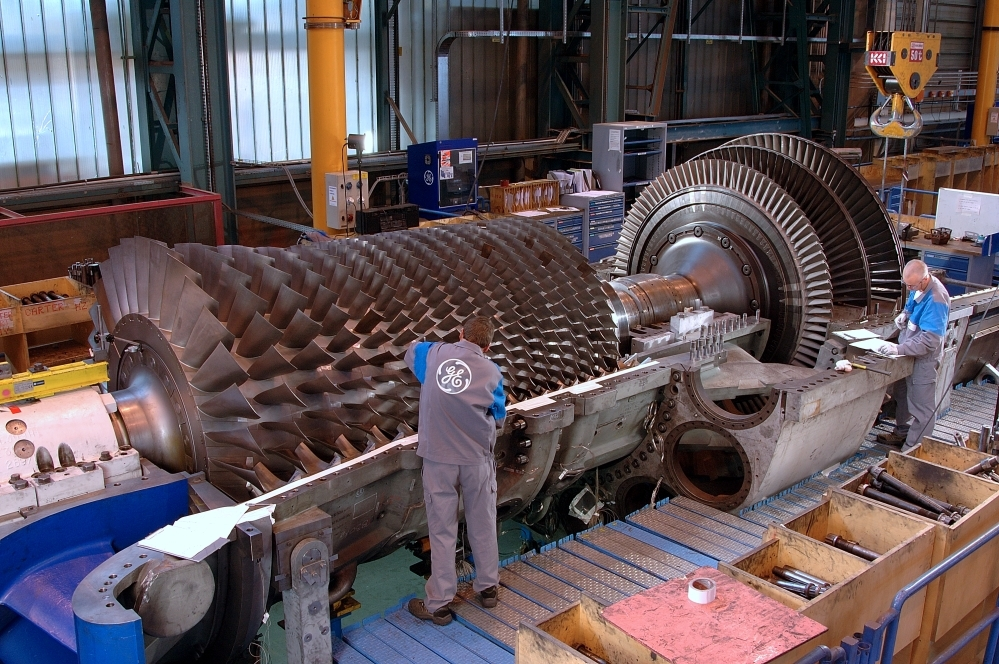
\includegraphics[width=.9\textwidth]{fig/TurboGas.png}
\caption{}
\label{fig:TurboGas}
\end{figure}

Per vedere come si presenta una turbina assiale si fa riferimento all'immagine in figura \ref{fig:TurboGas}, in cui è rappresentata una turbina a gas ad uso terrestre. Le pale hanno un'inclinazione di circa \ang{45}; la parte statorica avrà un grado di reazione di 0.5 ad eccezione del primo stadio e a monte potrebbe esserci un IGV. Sono presenti $17$ stadi di compressione e solo $3$ di turbina. 

Si analizzano quali possono essere le varie configurazioni di turbina richiamando nozioni del corso di Macchine:
\begin{itemize}
	\item stadi ad azione $R = 0$:
	\begin{align*}
	\begin{cases}
	\mbox{De laval} & z_v = 1\\
	\mbox{Reteau} & z_v = 1\\
	\mbox{Curtis} & z_v = 2 \div 3\\
	\end{cases}
	\end{align*}
	con $z_v$ salti di velocità. Lo stadio De Laval generalmente è usato nel primo stadio mentre lo stadio Reteau generalmente è usato nello stadio intermedio;
	\item stadi a reazione $R\neq 0$: turbine Parsons con $R = 0,5$.
\end{itemize}

Si possono determinare i triangoli di velocità:
\begin{align*}
\bigg( \frac{u}{c_1} \bigg)_{opt} = \frac{\sin \alpha_1}{2 z_v} \;\;\;\;\;\;\; \mbox{per} \; R = 0
\end{align*}
\begin{align*}
\bigg( \frac{u}{c_1} \bigg)_{opt} = \sin \alpha_1 \;\;\;\;\;\;\; \mbox{per} \; R = 0,5
\end{align*}
Essendo $\alpha_1$ piccolo si può scrivere $ \sin \alpha_1 \simeq \alpha_1$ semplificando ulteriormente le espressioni.

\section{Calcolo dei rendimenti}
Si analizza ora quello che succede all'interno dello stadio di una turbina. Ci si pone sul sistema di riferimento dato dalla linea media del condotto palare mostrato in \ref{fig:SezioneTurbina}. In questo caso non è più possibile assumere trascurabile la variazione di raggio. 
\begin{figure}
\centering
\begin{minipage}{.5\textwidth}
  \centering
  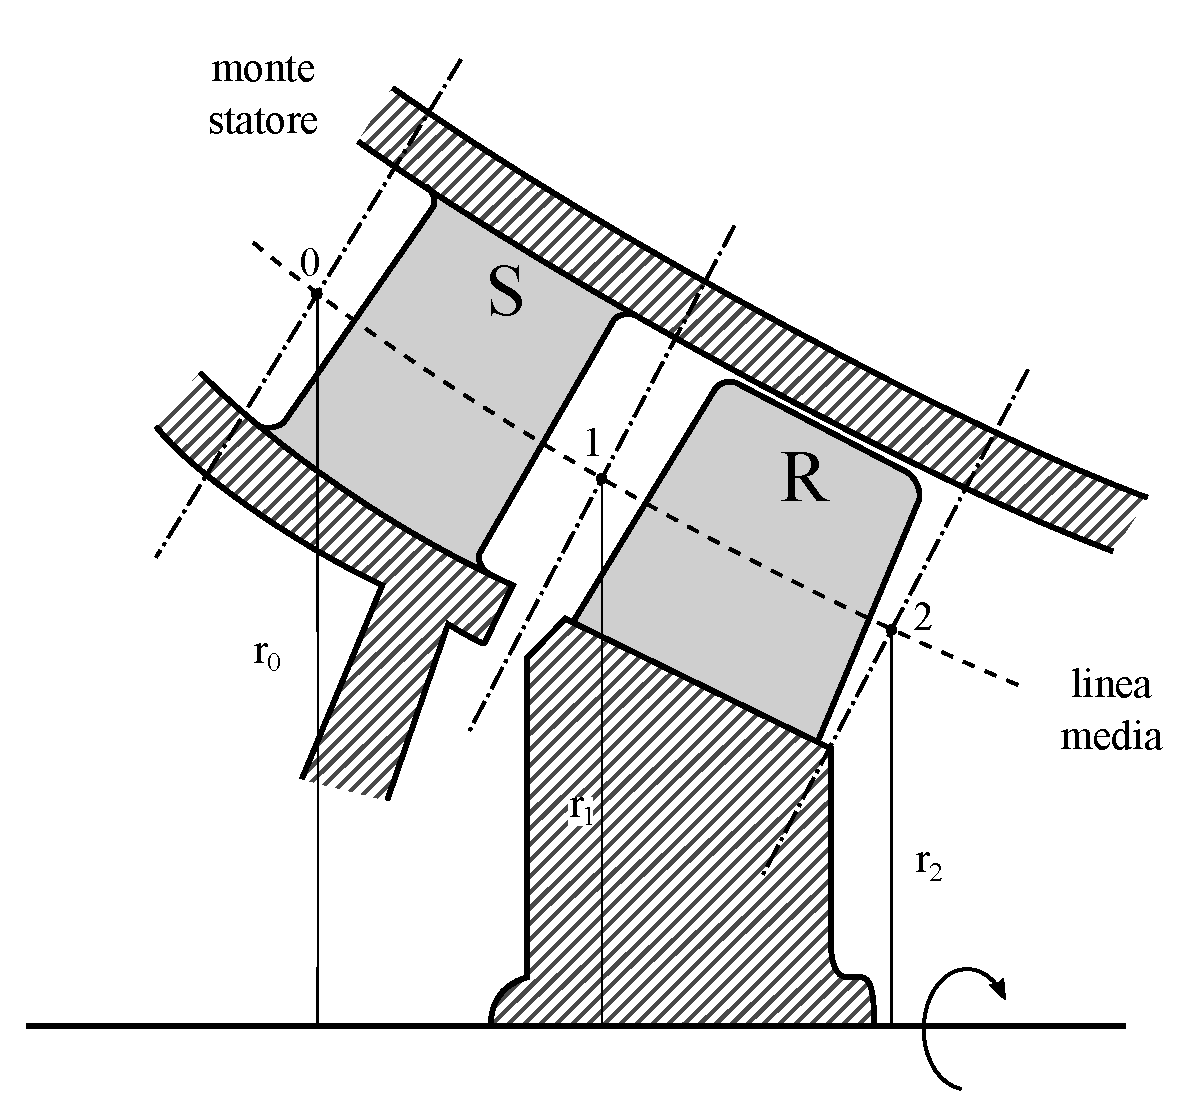
\includegraphics[width=.95\linewidth]{fig/SezioneTurbina.pdf}
  \captionof{figure}{}
  \label{fig:SezioneTurbina}
\end{minipage}%
\begin{minipage}{.5\textwidth}
  \centering
  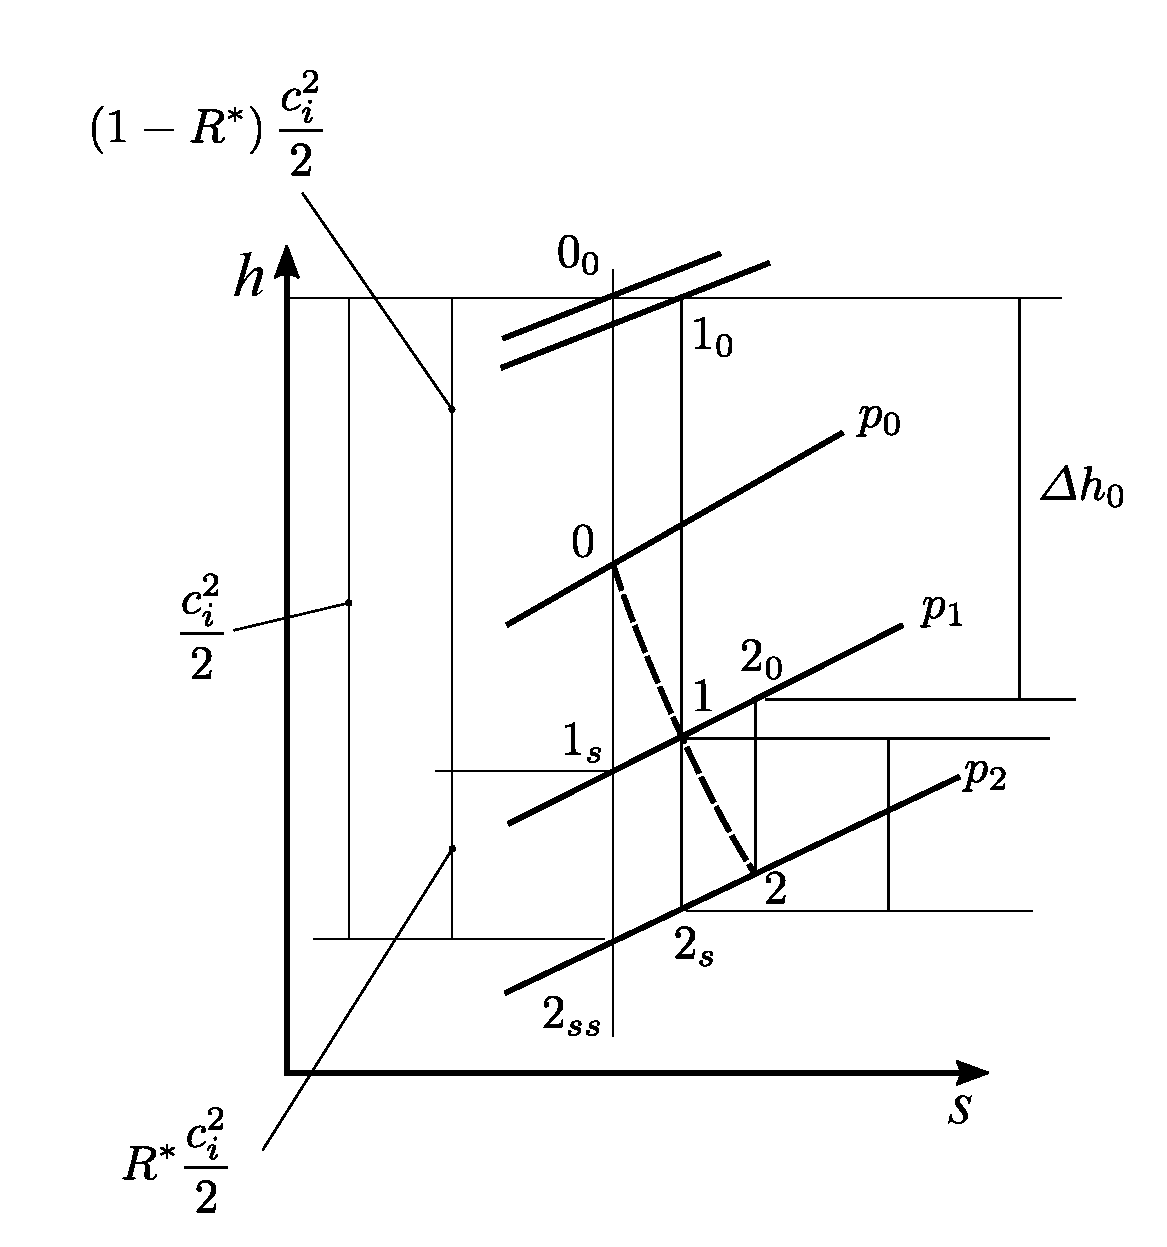
\includegraphics[width=.95\linewidth]{fig/hsturbine.pdf}
  \captionof{figure}{}
  \label{fig:hsturbine}
\end{minipage}
\end{figure}
\\Il salto entalpico tra i punti $1 - 2_s$ è leggermente superiore a quello presente tra i punti $1_s - 2_{ss}$ a causa della divergenza delle isobare. A tal proposito si introduce il fattore di recupero $f$. Questo fattore di recupero è fisicamente spiegabile dal fatto che la trasformazione, non essendo puramente isoentropica, causa un aumento della temperatura che verrà parzialmente recuperato nell'attraversamento successivo. 
\begin{center}
\begin{tabular}{l l l l l}
	$R^* \cdot \cfrac{c_i^2}{2}$ &&&& salto entalpico tra $1_s$ e $2_{ss}$\\
	$(1+f)R^* \cdot \cfrac{c_i^2}{2}$ &&&& salto entalpico tra $1$ e $2_s$\\
\end{tabular}
\end{center}
\subsection{Rendimenti}
Il rendimento è il seguente:
\begin{align*}
\eta = \cfrac{h_{0_0} - h_{2_0}}{h_{0_0} - h_{2_{ss}} - \Phi_E \cfrac{c_2^2}{2}} = \frac{\Delta h_0}{\Delta h_{is_{ts}}-\Phi_E \cfrac{c_2^2}{2}}
\end{align*}
con il termine $\Phi_E$ che rappresenta la quota cinetica a valle della turbina:
\begin{itemize}
	\item se $\Phi_E=1$ si considera un rendimento \textit{Total to Total} ($\eta \equiv \eta_{tt}$);
	\item se $\Phi_E=0$ si considera un rendimento \textit{Total to Static} ($\eta \equiv \eta_{ts}$).
\end{itemize}
Seguono ora una serie di definizioni:\\
\renewcommand\arraystretch{3}
\begin{tabular}{l l l l l}
	Coefficiente di portata: & & & &  $\Phi_1 = \cfrac{c_{m1}}{u_1}$\\
	Grado di reazione ideale: & & & & $R^* = \cfrac{h_{1s} - h_{2ss}}{h_{0_0} - h_{2_{ss}}} = \cfrac{\Delta h_{R_{is}}}{\Delta h_{is_{ts}}}$\\
	Energia cinetica totale: & & & &  $\cfrac{c_i^2}{2}=h_{0_0} - h_{2_{ss}}$\\
	Coefficiente di lavoro specifico ideale: & & & &  $\psi = \cfrac{h_{0_0} - h_{2_{ss}}}{\cfrac{u_1^2}{2}} = \cfrac{\Delta h_{is_{ts}}}{\cfrac{u_1^2}{2}}= \cfrac{c_i^2}{u_1^2}$\\
	Coefficiente di lavoro specifico reale: & & & &  $\lambda = \cfrac{h_{0_0} - h_{2_0}}{\cfrac{u_1^2}{2}}= \cfrac{\Delta h_0}{\cfrac{u_1^2}{2}}$\\
	Coefficiente di velocità periferica: & & & &  $k_{is} = \cfrac{u_1}{c_i} = \cfrac{1}{\sqrt{\psi}}$\\
\end{tabular}

\vspace{0.5cm}
Dopo aver adimensionalizzato i triangoli di velocità non è più possibile riferirsi ad una sola velocità meridiana in quanto questa diventa una grandezza di progettazione visto che definisce le sezioni della macchina; si usano quindi i rapporti tra velocità meridiane e tra i raggi:
\begin{align*}
\frac{c_{m2}}{c_{m1}} \;\; \text{e} \;\; \frac{r_2}{r_1}
\end{align*}
Si adimensionalizzano tutte le grandezze con la velocità periferica $u_1$. Chiaramente i triangoli di velocità saranno di dimensioni diverse come mostrato in figura \ref{fig:triangTurb}. 
\begin{figure}[h!]
\centering
  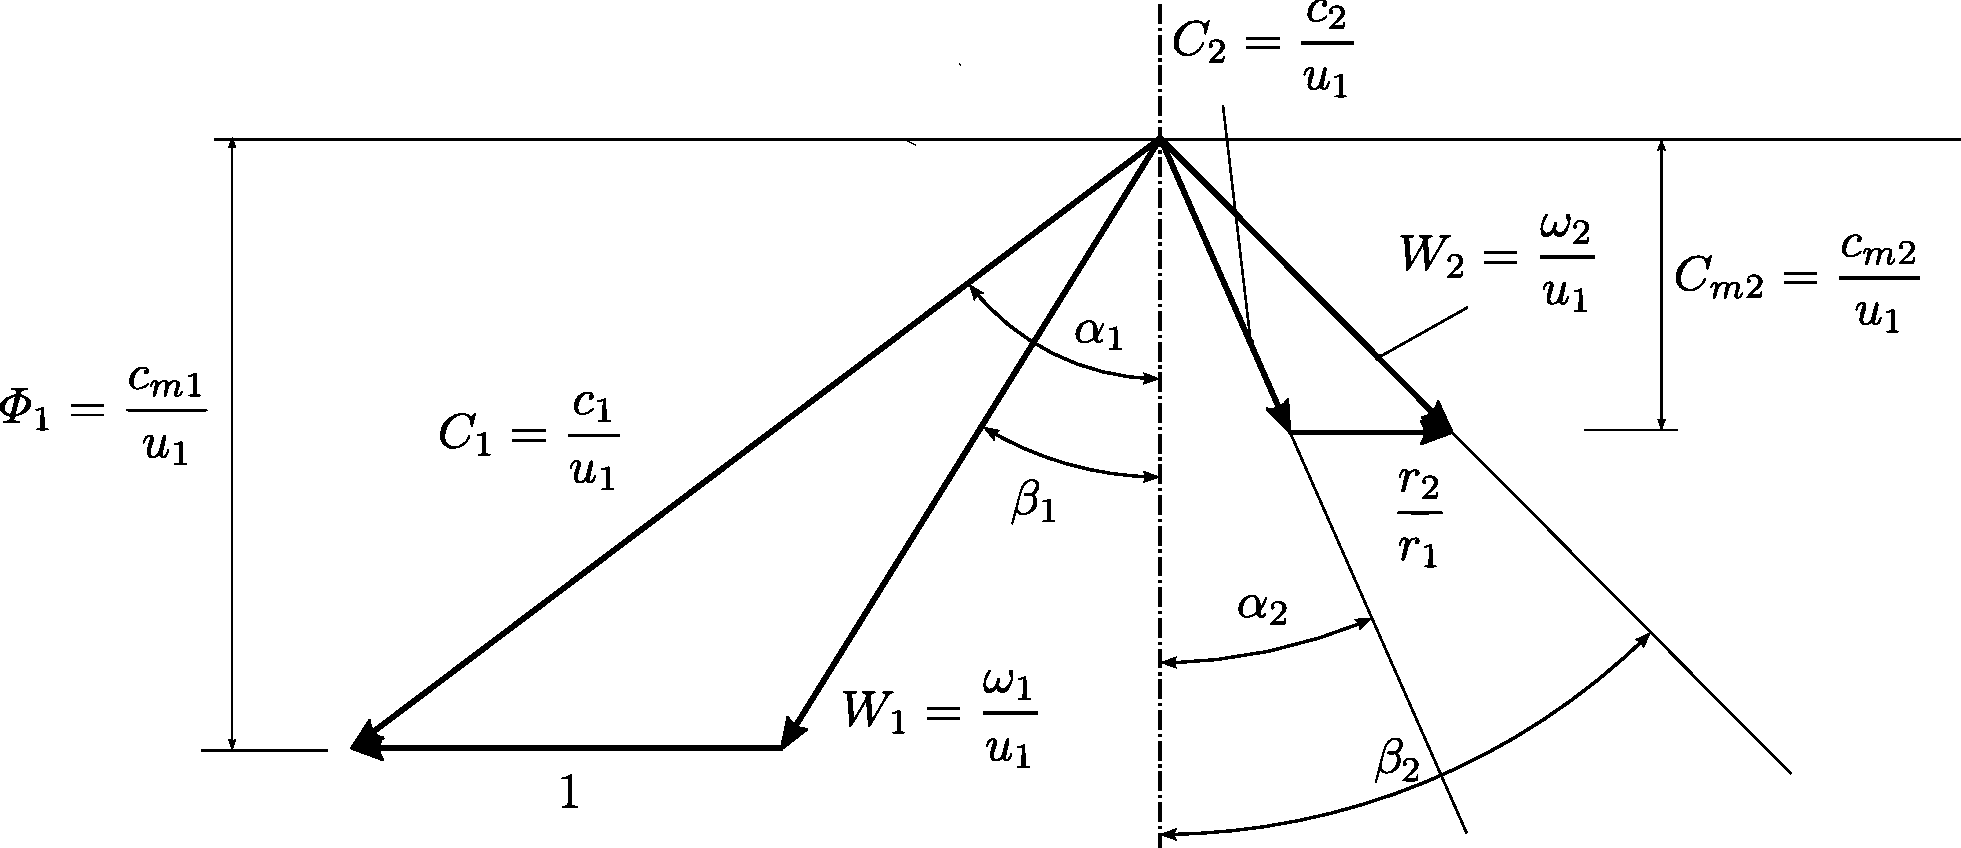
\includegraphics[width=.8\textwidth]{fig/triangTurb.pdf}
\caption{}
\label{fig:triangTurb}
\end{figure}
\\\'E possibile andare ora a sviluppare l'espressione del rendimento:
\begin{equation}
\eta = \cfrac{\Delta h_0}{\Delta h_{is_{ts}} - \Phi_E \cfrac{c_2^2}{2}} \cdot \frac{\frac{1}{u_1^2/2}}{\frac{1}{u_1^2/2}} = \frac{\lambda}{\psi - \Phi_E \left( C_2^2 \right)}
\end{equation}
con a numeratore
\begin{align*}
\lambda = \cfrac{\Delta h_0}{\cfrac{u_1^2}{2}} = \frac{2 \left( u_1 c_{u1} - u_2 c_{u2} \right)}{u_1^2} = 2 \bigg( C_{u1} - \frac{r_2}{r_1} C_{u2} \bigg)
\end{align*}
Si scrivono ora le velocità assolute adimensionalizzate, $C_i$, in funzione del rendimento e del grado di reazione:
\begin{align*}
\frac{c_1^2}{2} = \left( 1 - R^* \right) \frac{c_i^2}{2} \cdot \eta_s \;\;\;\; \Rightarrow \;\;\;\; c_1 = \sqrt{\eta_s \left( 1 - R^* \right)} \cdot c_i
\end{align*}
\begin{align*}
C_1 = \frac{c_1}{u_1} = \sqrt{\eta_s \left(1- R^* \right)} \cdot \frac{c_i}{u_1} \hspace{0.5cm} \mbox{con } \frac{c_i}{u_1} = \frac{1}{k_{is}}
\end{align*}
Risulta
\begin{equation}
\boxed{ C_1 = \frac{\sqrt{\eta_s}}{k_{is}} \sqrt{1 - R^*} }
\end{equation}
Si procede con la stessa operazione per le altre grandezze.

Per esprimere la velocità relativa adimensionalizzata $W_1$ si usa il teorema di Carnot:
\begin{align*}
W_1^2 = C_1^2 + 1^2 - 2 \cdot 1 \cdot C_1 \cos \cdot \big( \frac{\pi}{2} - \alpha_1 \big)
\end{align*}
ottenendo
\begin{equation}
\boxed{ W_1 = \sqrt{1 + \frac{\eta_{s}}{k_{is}^2} \left( 1 - R^* \right) - 2 \frac{\sqrt{\eta_s}}{k_{is}} \sqrt{1-R^*} \cdot \sin \alpha_1}}
\label{eq:W1}
\end{equation}

Per quanto riguarda $W_2$, si considera il salto entalpico e lo si esprime in funzione del fattore di recupero $f$:
\begin{equation}
h_2 - h_1 = \frac{u_2^2 - u_1^2}{2} - \frac{w_2^2 - w_1^2}{2}
\end{equation}
\begin{align*}
h_1 - h_2 = \frac{c_i^2}{2} \cdot R^* \left( 1 + f \right) \eta_R
\end{align*}
\begin{align*}
\Bigg[\frac{w_2^2 - w_1^2}{2} - \frac{u_2^2 - u_1^2}{2} = \frac{c_i^2}{2} \cdot R^* \left( 1 + f \right) \eta_R \Bigg] \cdot \frac{1}{u_1^2}
\end{align*}
\begin{equation}
\boxed{W_2 = \sqrt{\frac{\eta_R \left( 1 + f \right) R^*}{k_{is}^2} + \frac{\eta_s}{k_{is}^2}  \left(1 - R^* \right) - \frac{2 \sqrt{\eta_s}}{k_{is}} \sqrt{1 - R^*} \sin \alpha_1 + \bigg(\frac{r_2}{r_1} \bigg)^2 } }
\end{equation}
\\Per quanto riguarda $C_{m2}$:
\begin{align*}
c_{m2} = c_{m1} \frac{c_{m2}}{c_{m1}}=c_1 \cos \alpha_1 \cdot \frac{c_{m2}}{c_{m1}}
\end{align*}
\begin{align*}
C_{m2} = C_1 \cos \alpha_1 \cdot \frac{c_{m2}}{c_{m1}}
\end{align*}
ottenendo
\begin{equation}
\boxed{C_{m2} = \frac{c_{m2}}{c_{m1}} \frac{\sqrt{\eta_s}}{k_{is}} \sqrt{1 - R^*} \cos \alpha_1 }
\end{equation}
In questo modo è possibile scrivere il rendimento come funzionale di tutte le grandezze viste :
\begin{align*}
\boxed{\eta = f \bigg( \psi, \Phi_E, R^*, k_{is}, f, \frac{c_{m2}}{c_{m1}}, \frac{r_2}{r_1}, \alpha_1, \eta_s, \eta_R \bigg)}
\end{align*}
I primi quattro parametri sono parametri funzionali, $f$ dipende dalla divergenza delle isobare e quindi dalla natura del fluido, i tre parametri successivi sono parametri di progetto e infine gli ultimi due sono parametri della schiera rotorica e statorica.\\
\'E possibile tracciare un diagramma di rendimento Total to Static / Total to Total in funzione del coefficiente di lavoro specifico ideale (figura \ref{fig:Rendimenti_ts_tt}). 
\begin{figure}
\centering
  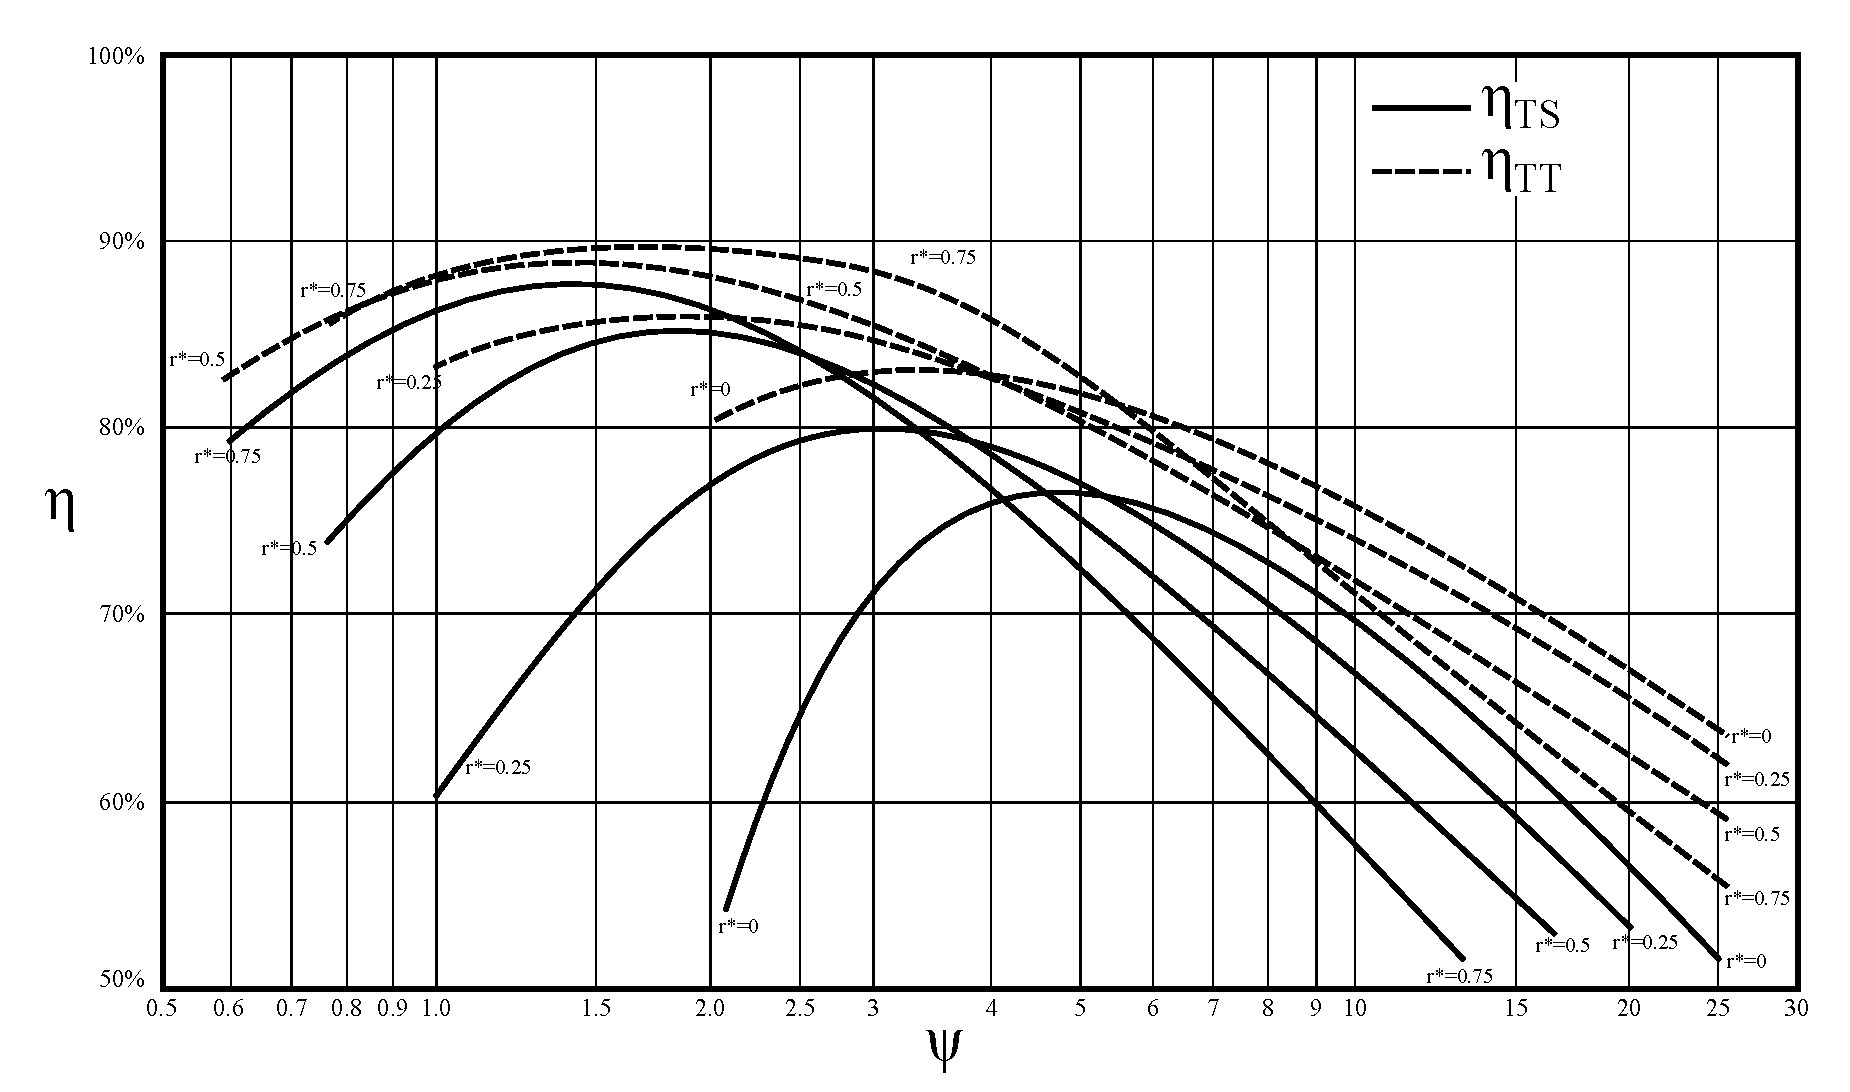
\includegraphics[width=.8\textwidth]{fig/Rendimenti_ts_tt.pdf}
\caption{}
\label{fig:Rendimenti_ts_tt}
\end{figure}
\section{Proprietà termodinamiche del flusso}
Si possono ora calcolare le proprietà termodinamiche del flusso nell'attraversamento della turbina. Si definisce il numero di Mach periferico come:
\begin{align*}
M_u = \frac{u_1}{a_{0_0}}
\end{align*}
\'E possibile esprimere la velocità acustica a monte della turbina in funzione dell'entalpia totale:
\begin{align*}
a_{0_0} = \sqrt{kRT_{0_0}} = \sqrt{\frac{c_p}{c_v} \left( c_p - c_v \right) T_{0_0}} = \sqrt{h_{0_0} \left( k - 1 \right)}
\end{align*}
e
\begin{align*}
\psi = \cfrac{h_{0_0} - h_{2ss}}{\cfrac{u_1^2}{2}} = \cfrac{\Delta h_{is_{ts}}}{\cfrac{u_1^2}{2}} = \cfrac{c_i^2}{u_1^2} \hspace{2cm} \frac{c_i^2}{2} = \psi \frac{u_1^2}{2} \cdot \frac{a_{0_0}^2}{a_{0_0}^2} = \frac{k-1}{2}\psi {M_u}^2 h_{0_0}
\end{align*}
Si ricavano quindi le espressioni dei punti delle trasformazioni isoentropiche:
\begin{align*}
h_{1s} = h_{0_0} - \left(1- R^* \right) \frac{c_i^2}{2} = h_{0_0} \bigg[ 1- \left( 1- R^* \right) \frac{k-1}{2} \psi M_u^2 \bigg]
\end{align*}
\begin{align*}
h_{2ss} = h_{0_0} - \frac{c_i^2}{2} = h_{0_0} \bigg[ 1 - \frac{k-1}{2} \psi M_u^2 \bigg]
\end{align*}
Ricordando che
\begin{align*}
\frac{c_1^2}{2} = \frac{c_i^2}{2} \left( 1- R^* \right) \eta_s
\end{align*}
si arriva alle espressioni dell'entalpia nei punti $1$ e $2$:
\begin{align*}
\boxed{h_1 = h_{0_0} - \frac{c_1^2}{2} = h_{0_0} \bigg[ 1- \left( 1- R^* \right) \frac{k-1}{2}  \psi M_u^2 \eta_s\bigg]}
\end{align*}
\begin{align*}
\boxed{h_2 = h_{0_0} - \Delta h_0 - \frac{c_2^2}{2} = h_{0_0} \bigg[ 1- \bigg( \eta_{ts} + \frac{C_2^2}{\psi} \bigg) \frac{k-1}{2} \psi M_u^2 \bigg]}
\end{align*}

\section{Schiere palari}
L'attraversamento del fluido attraverso la palettatura comporta una situazione meno critica dal punto di vista fluidodinamico rispetto il caso dei compressori. Il gradiente di pressione infatti, naturalmente non favorisce la separazione di vena fluida e perciò non sussistono grosse criticità sotto questo punto di vista permettendo di ottenere rendimenti più alti più facilmente. La deflessione imposta sarà quindi di gran lunga maggiore di quella del compressore e ne conseguiranno anche spessori maggiori. 
\begin{figure}
\centering
  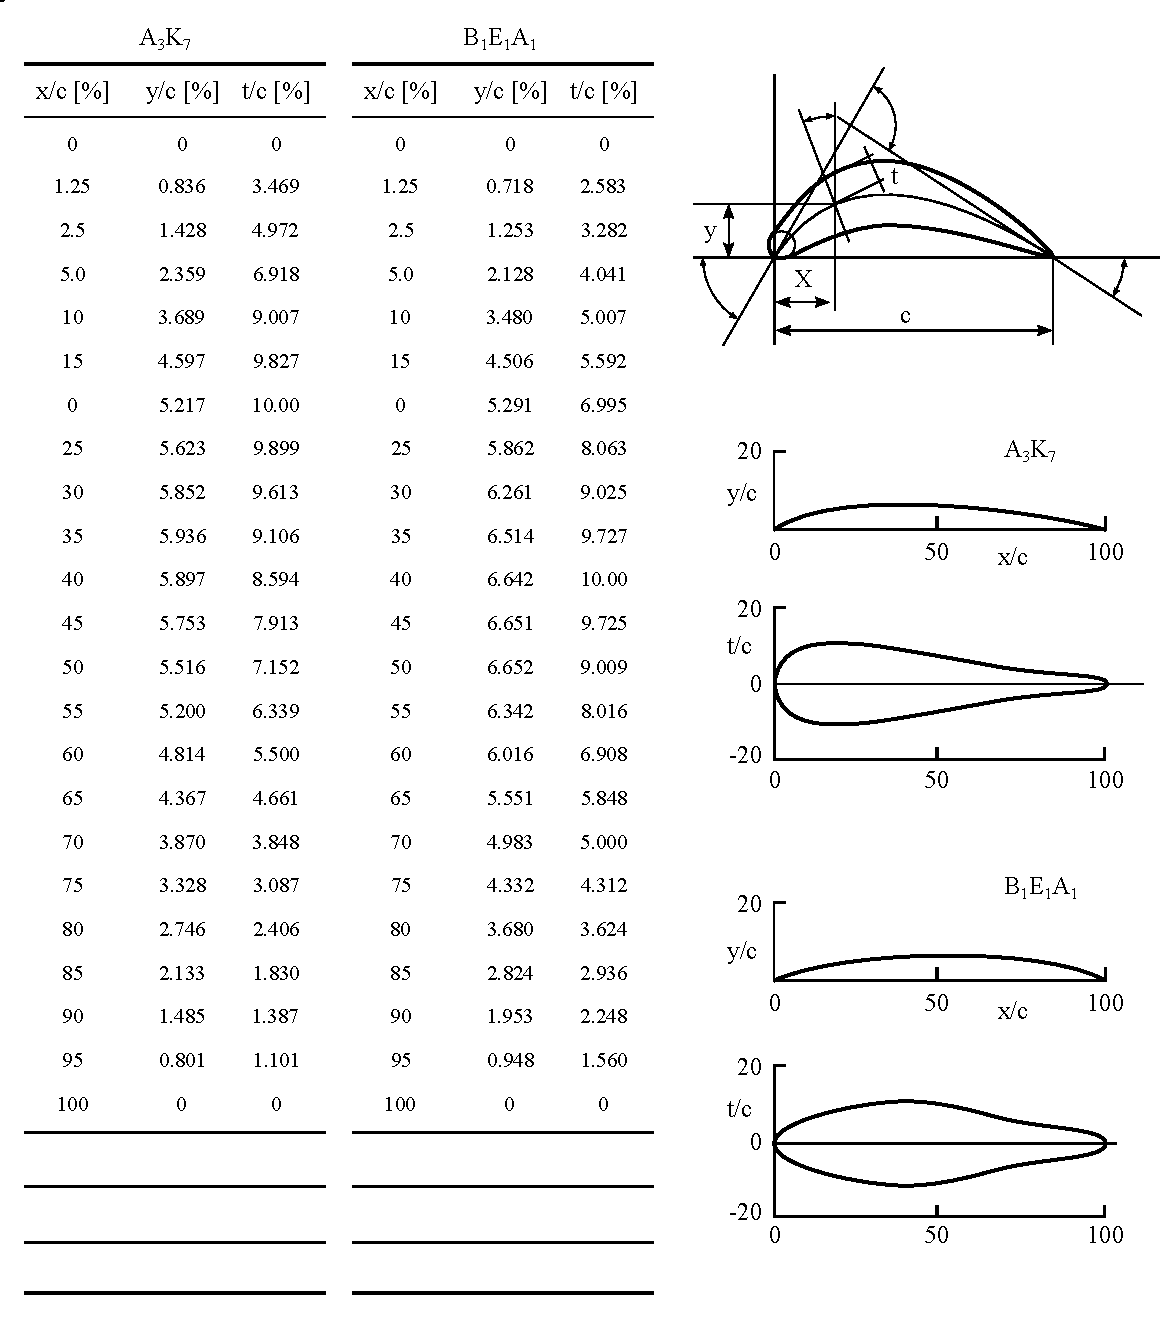
\includegraphics[width=\textwidth]{fig/SchierePaleTab.pdf}
\caption{}
\label{fig:SchierePaleTab}
\end{figure}

I profili a deflessione relativamente bassa, come quelli delle turbine a gas, si ricavano dalla somma di una distribuzione di spessori ad una linea media. Ci sono profili di diversa categoria e i valori sono ricavati in base a dei parametri di progettazione come mostrato in figura \ref{fig:SchierePaleTab}.

Nei profili ad alta deflessione, utilizzati soprattutto in macchine ad azione, la sezione è costituita da una carenatura ad arco di cerchio. Come si vede in figura \ref{fig:palaBassaDef}, la componente $w_1$ ha stesso modulo di $w_2$ e vi è semplicemente una deviazione nella direzione del secondo vettore. La palettatura è un arco di cerchio tangente alle due direzioni e presenta un inspessimento verso il centro per dare maggiore resistenza meccanica. La coda è tronca mentre il leading edge non può naturalmente esserlo e per questo viene arrotondato. 
\begin{figure}
\centering
  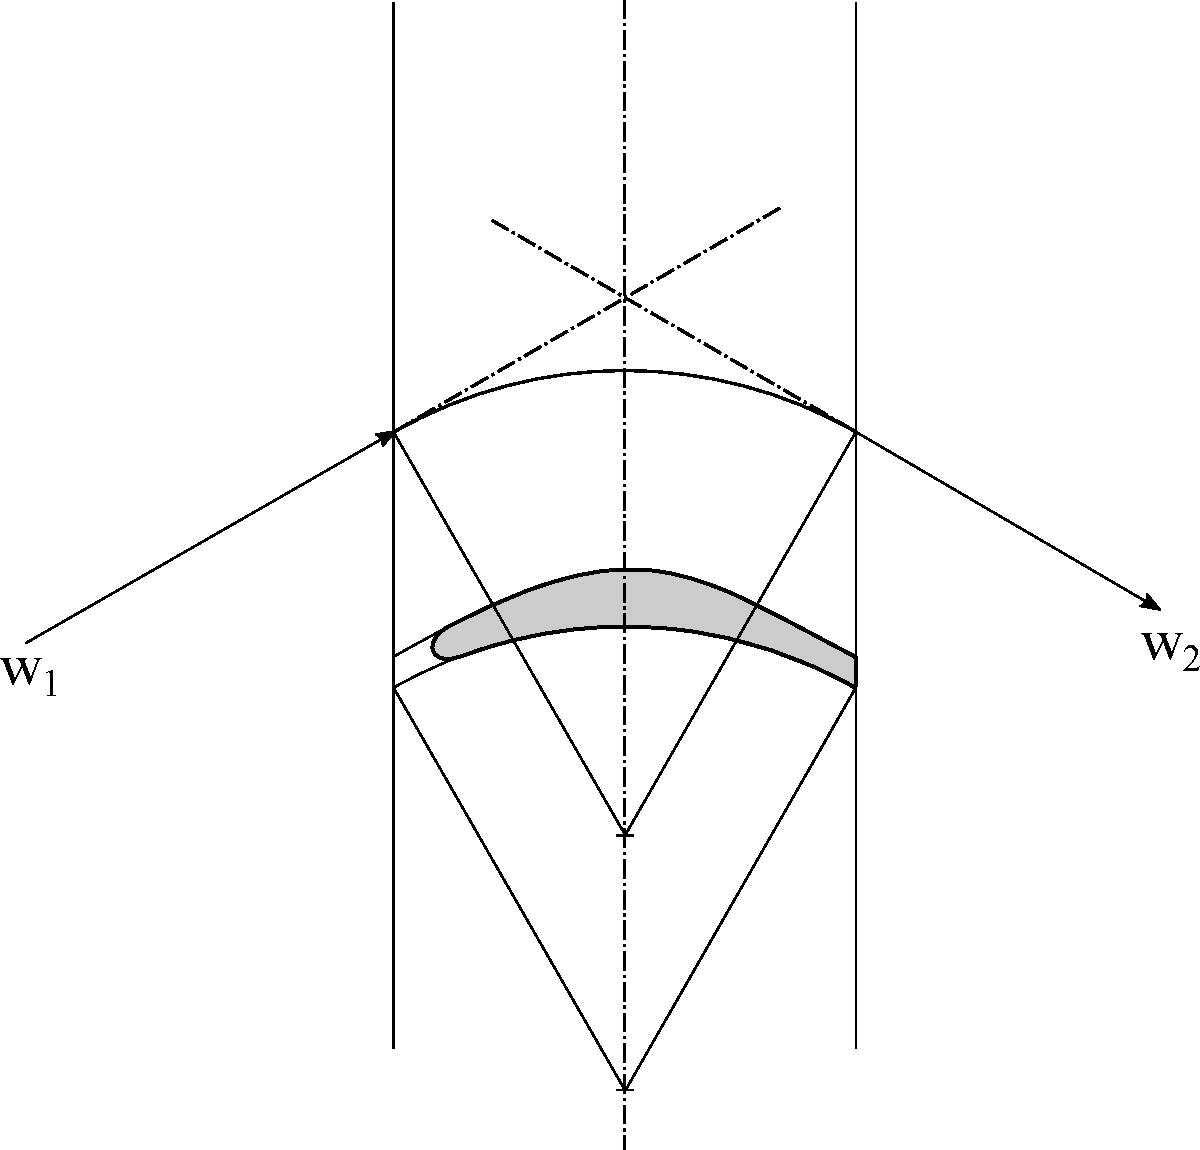
\includegraphics[width=.6\textwidth]{fig/palaBassaDef.pdf}
\caption{}
\label{fig:palaBassaDef}
\end{figure}

In alcuni casi, come con turbine a vapore, gli effetti di comprimibilità non sono trascurabili.\\
Come si può notare osservando la figura \ref{fig:SupSonic} in alto, nel caso sia presente un flusso subsonico si forma sul dorso del profilo isolato una zona supersonica con una discontinuità data da un'onda d'urto.\\
Osservando invece la figura \ref{fig:SupSonic} in basso, nel caso il flusso sia supersonico si verifica la formazione di un'onda d'urto prima del profilo isolato che porta quindi ad un incremento della sua resistenza al flusso; a valle si formano invece delle onde d'urto oblique.

Considerando un insieme di pale in presenza di velocità supersonica del flusso, figura \ref{fig:PaleSup} a destra, a valle del condotto convergente si instaura un'onda d'urto e un sistema di onde oblique che va ad interagire con la palettatura del rotore posta a valle. \'E possibile distinguere un'onda normale sul condotto (a) e un'onda obliqua a valle (b). Si tratta di un sistema complicato di onde d'urto. Per stabilizzare il comportamento della palettatura si utilizzerà quindi un leading edge appuntito.
\begin{figure}
\centering
\begin{minipage}{.5\textwidth}
  \centering
  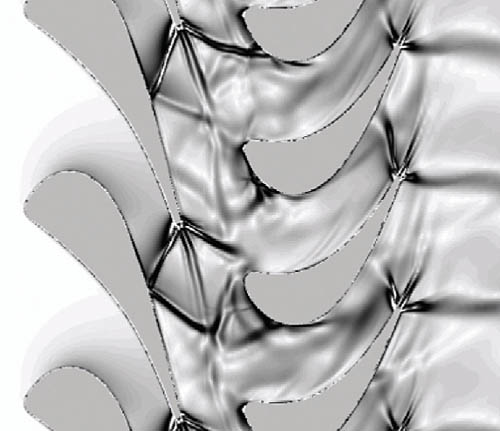
\includegraphics[width=.95\linewidth]{fig/ou_schiera.png}
  \captionof{figure}{}
  \label{fig:ou_schiera}
\end{minipage}%
\begin{minipage}{.5\textwidth}
  \centering
  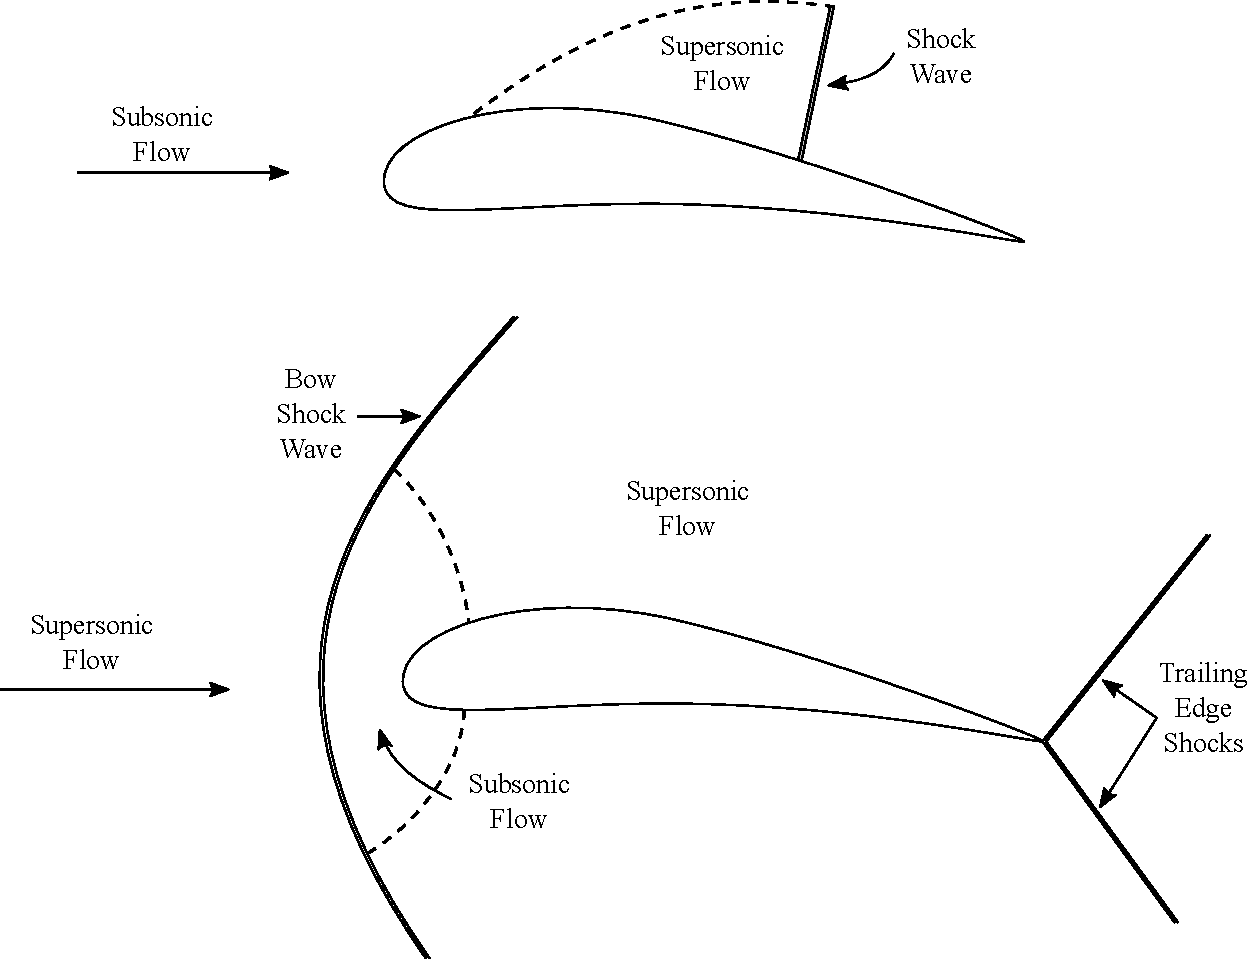
\includegraphics[width=.95\linewidth]{fig/SupSonic.pdf}
  \captionof{figure}{}
  \label{fig:SupSonic}
\end{minipage}
\end{figure}
\begin{figure}
\centering
  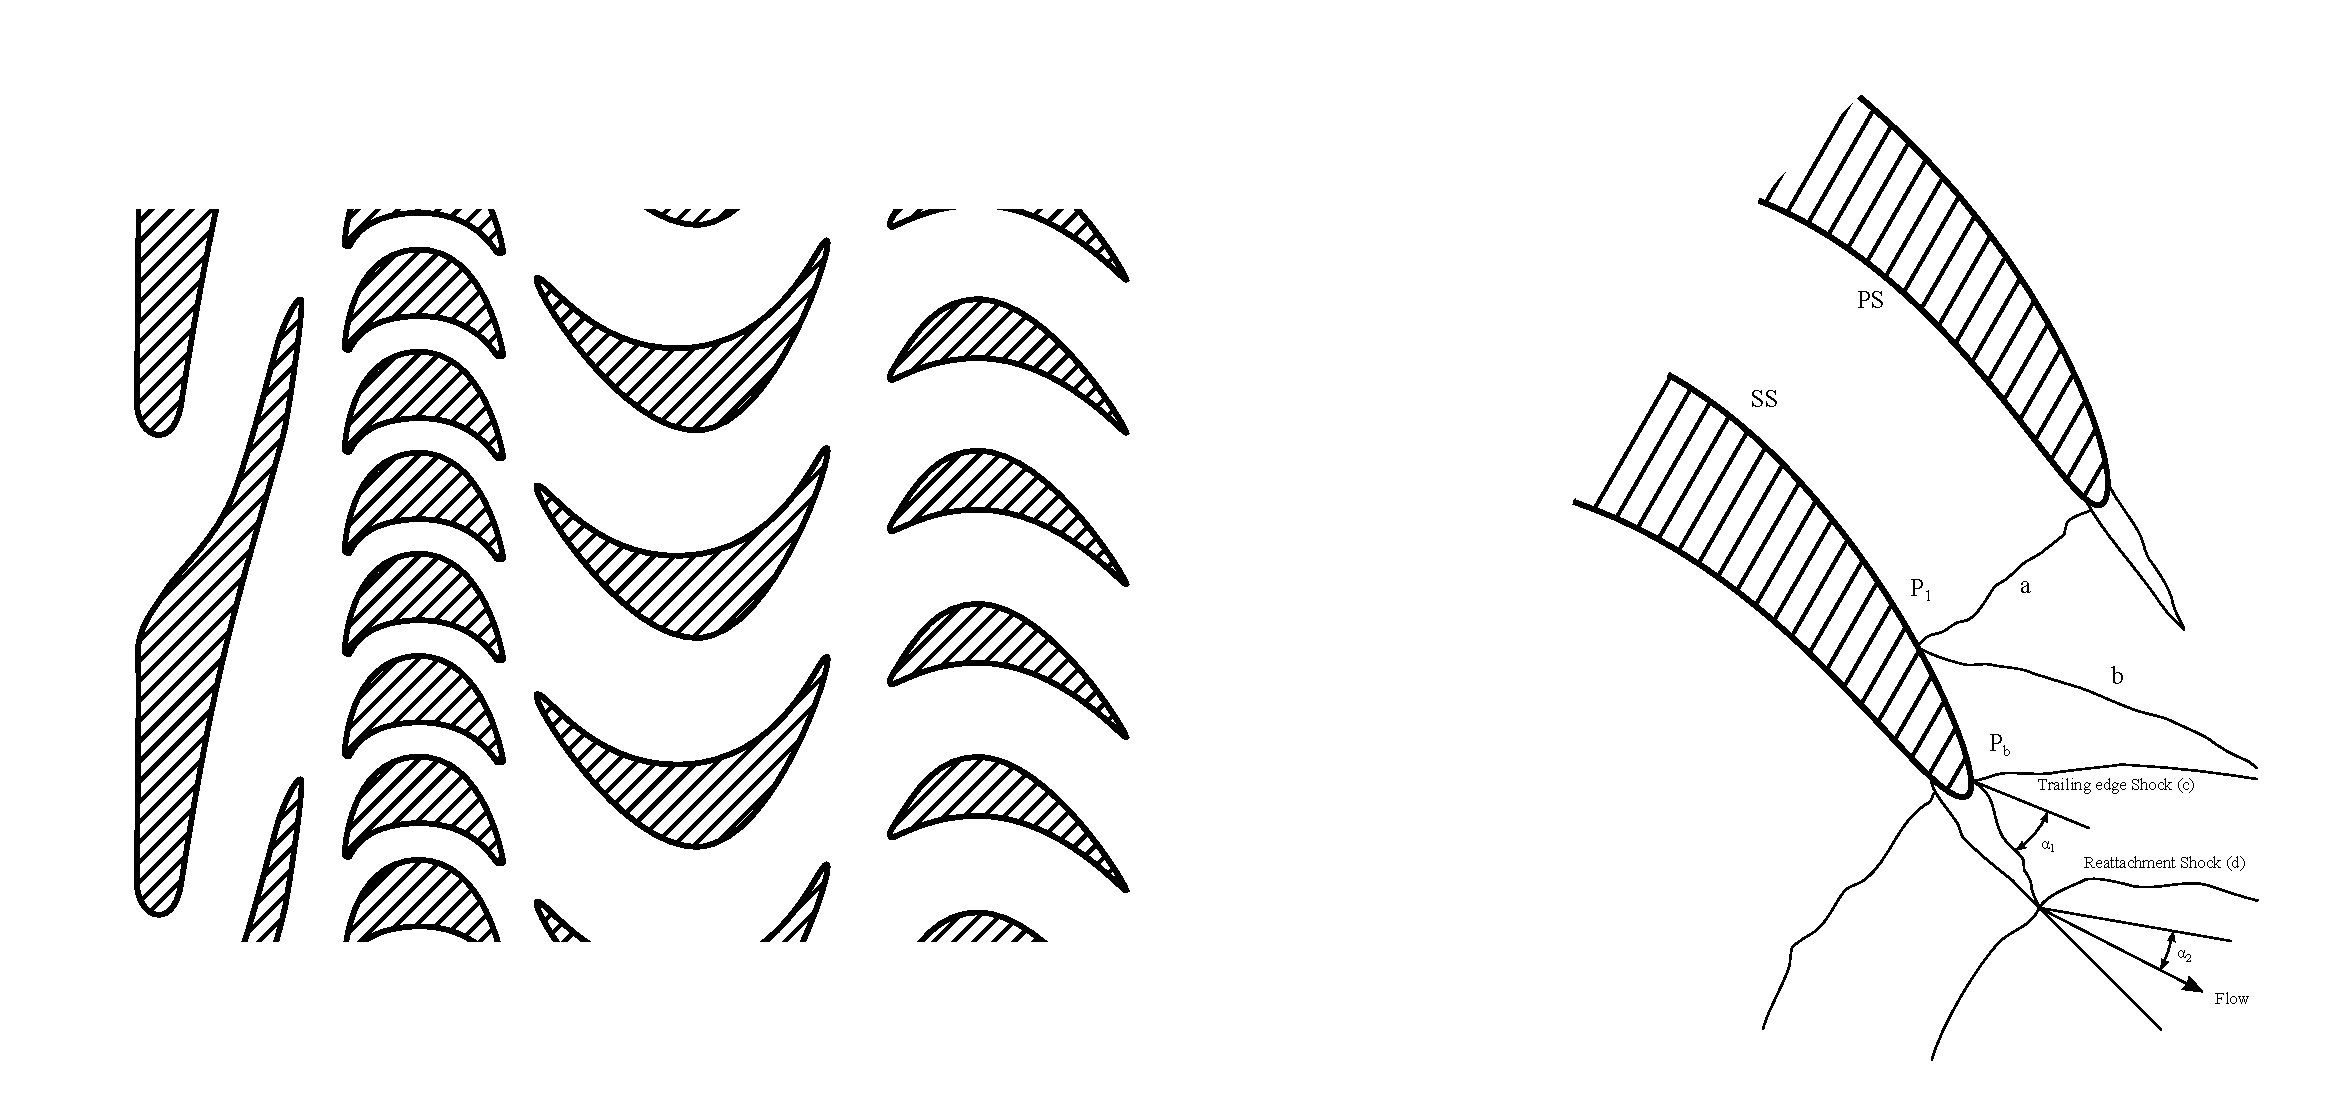
\includegraphics[width=\textwidth]{fig/PaleSup.pdf}
\caption{}
\label{fig:PaleSup}
\end{figure}

\section{Prestazioni della schiera}
Definiti i triangoli di velocità si cerca ora il coefficiente di perdita in uscita e l'angolo in uscita. In prima approssimazione si possono trascurare $Ma$ e $Re$.
\begin{figure}[h!]
\centering
  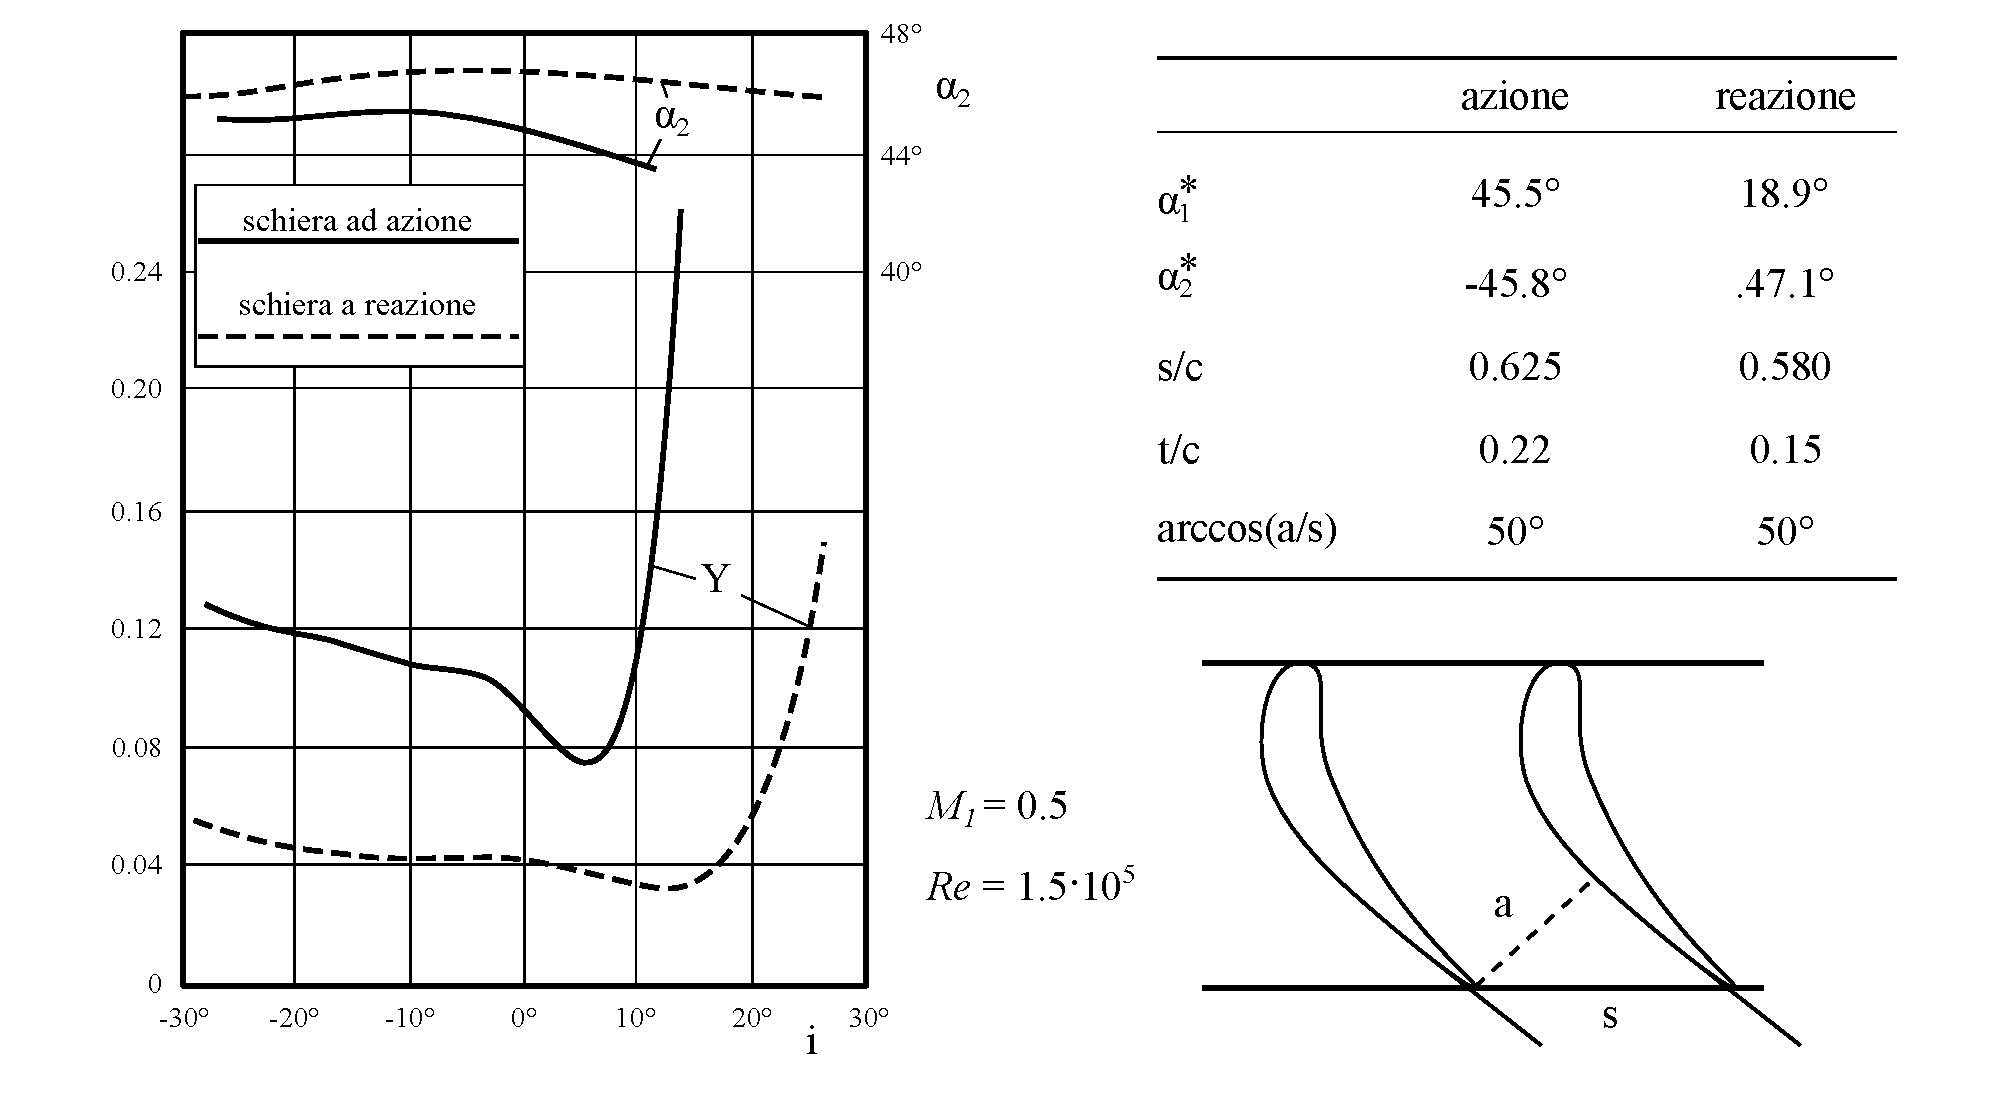
\includegraphics[width=\textwidth]{fig/PrestSchieraTurb.pdf}
\caption{}
\label{fig:PrestSchieraTurb}
\end{figure}

Stabilire l'angolo del fluido in uscita non è ovvio: in presenza di una deviazione elevata della palettatura è presente un ampio passo palare. Per definire l'angolo di deviazione in uscita si considera la normale al ventre del profilo dal trailing edge e il passo palare, figura \ref{fig:PrestSchieraTurb} in basso a destra, e quindi si ricava:
\begin{align*}
\alpha_2^* = \arccos \bigg(\cfrac{a}{s}\bigg)
\end{align*}
$\alpha_2$ è poco variabile al variare dell'incidenza; si rileva un comportamento abbastanza costante anche per il primo tratto del coefficiente di perdita.

\'E noto che l'angolo di flusso non sarà esattamente pari all'angolo di pala:
\begin{align*}
\cos \alpha_1 = \frac{1}{k} \cos \alpha_1^*
\end{align*}
dove $k$ può essere stimato con diverse correlazioni sperimentali. Un esempio di correlazione per il calcolo di $k$ è quella di \textit{Vaura}:
\begin{align*}
k = 1 - 10750 \bigg( \frac{t}{s} \bigg)^{3.3} \bigg( \frac{a}{s} \bigg)
\end{align*}
in cui $t$ è lo spessore della pala all'uscita.

Per quanto riguarda le perdite, è possibile considerare la cumulata delle diverse perdite come mostrato in figura \ref{fig:PerditeSchiera} oppure utilizzare alcune correlazioni. 
\begin{figure}
\centering
  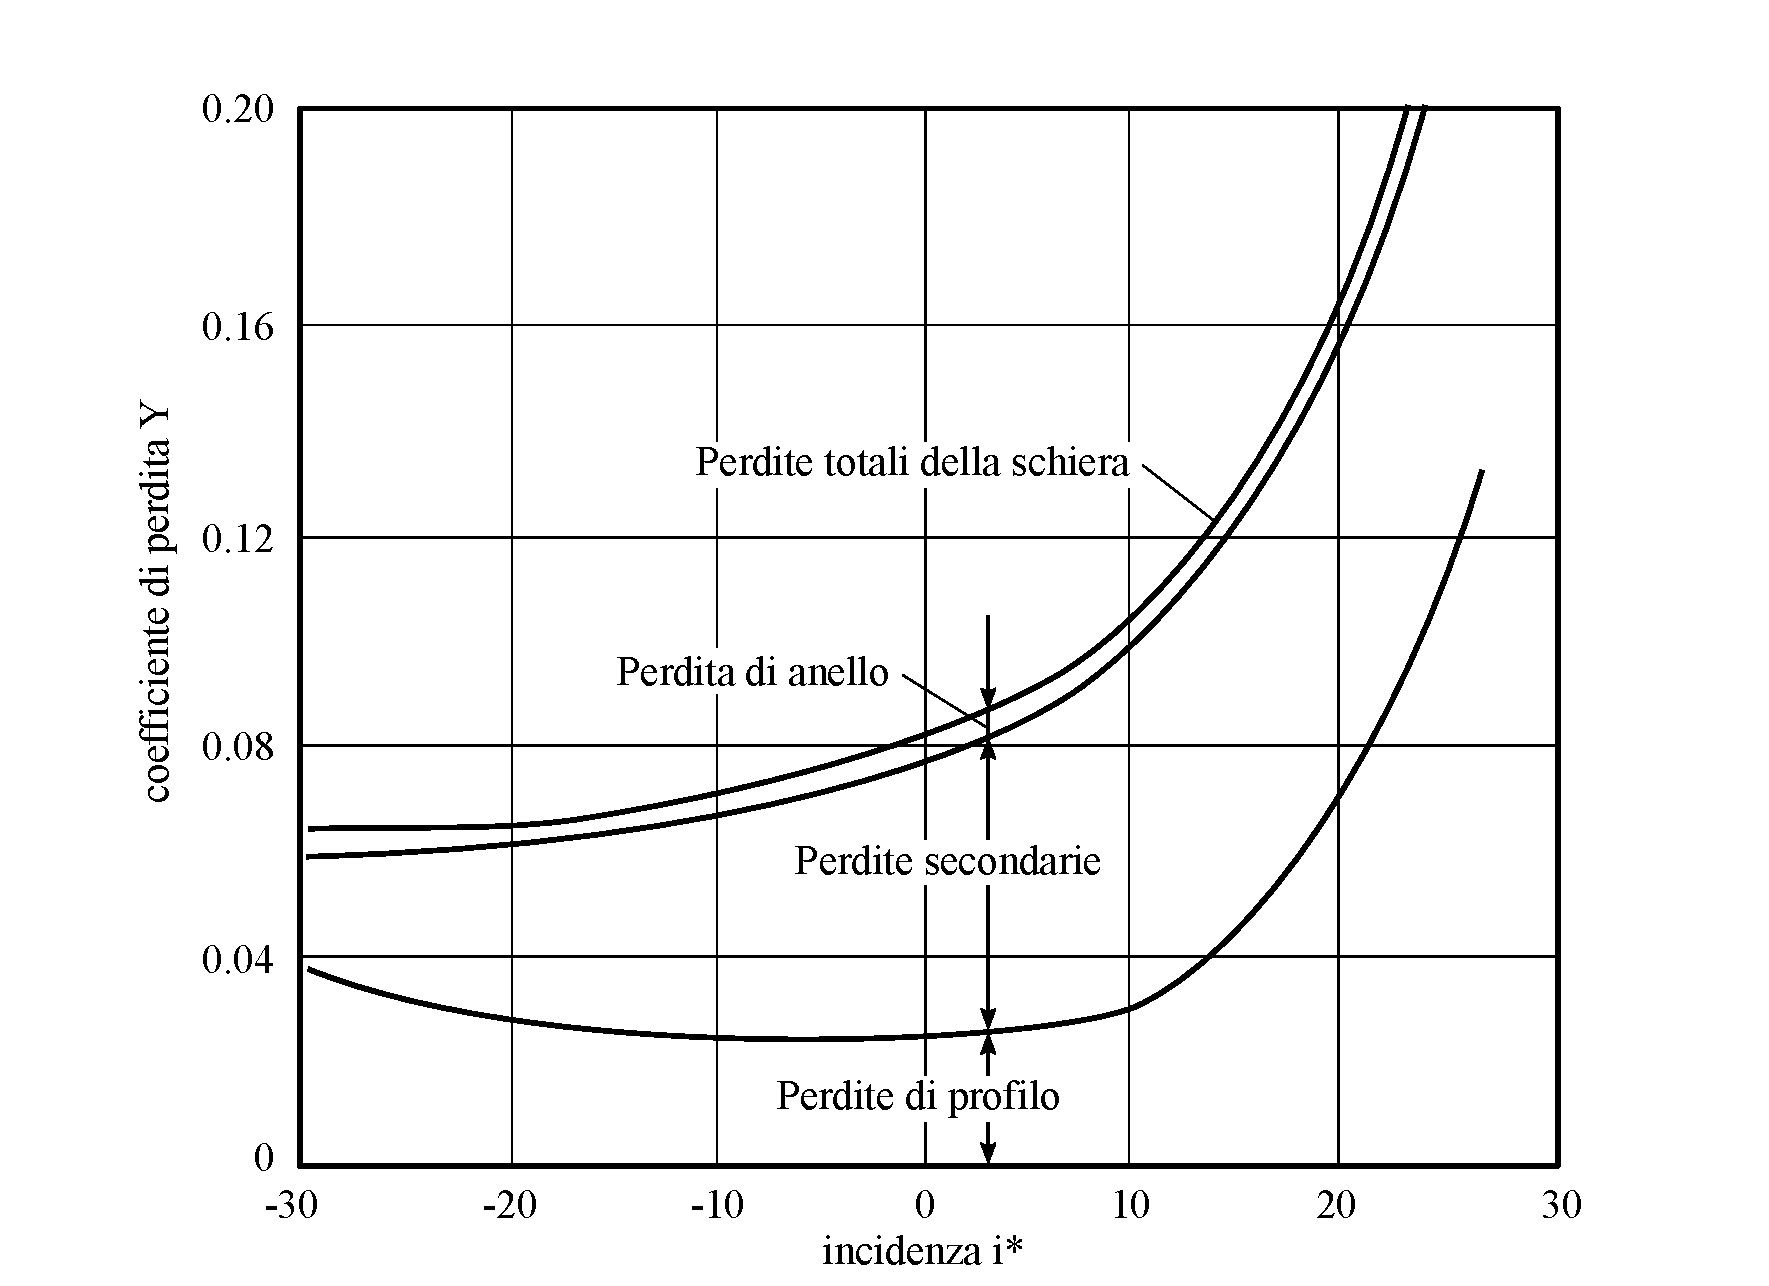
\includegraphics[width=.65\textwidth]{fig/PerditeSchiera.pdf}
\caption{}
\label{fig:PerditeSchiera}
\end{figure}
\subsection{Soderberg}
La correlazione di Soderberg permette di determinare globalmente tutte le perdite. \'E applicabile se vengono rispettate due condizioni:
\begin{itemize}
	\item la schiera si trova in condizioni di progetto;
	\item la solidità deve essere calcolata con un criterio di ottimizzazione (in particolare con il criterio di carico di Zweifel).
\end{itemize}
I coefficienti di perdita di energia adimensionalizzati rispetto l'energia cinetica effettiva allo scarico della schiera considerata sono:
\begin{align*}
\begin{cases}
\xi_1 = \cfrac{|h_1 - h_{1s}|}{\cfrac{1}{2} c_1^2} & \mbox{ per lo statore }\\
\\
\xi_2 = \cfrac{|h_2 - h_{2s}|}{\cfrac{1}{2} w_2^2} & \mbox{per il rotore }
\end{cases}
\end{align*}
Si cercano ora dei coefficienti funzione di:
\begin{itemize}
\item deflessione cinematica: $\Delta \alpha$ statore, $\Delta \beta$ rotore;
\item numero di Reynolds: $Re = \cfrac{D_i c_1 }{\nu}$
con $D_i$ diametro idraulico della sezione\footnote{ Diametro bagnato dal fluido: \begin{align*}
D_{i} = \frac{2 h s \cos \alpha_1}{h + s \cos \alpha_1} \mbox{ per lo statore}, \;\; D_{i} = \frac{2 h s \cos \beta_2}{h + s \cos \beta_2} \mbox{ per il rotore}
\end{align*} con $h$ altezza della pala.};
\item allungamento della pala $h/b$;
\item $t_{max}/c$.
\end{itemize}
Le correlazioni sono espresse rispetto ad una perdita $\xi^*$ (figura \ref{fig:Soderberg}) in funzione della deflessione cinematica $\varepsilon$ al variare del rapporto $t_{max}/c$. Si tratta di una sintesi di dati sperimentali di una palettatura di riferimento ricavati in galleria del vento.
\begin{align*}
\begin{cases}
\xi = \bigg( \cfrac{10^5}{Re} \bigg)^{0.25} \bigg[ \left( 1 + \xi^* \right) \bigg ( 0.975 + 0.075 \cfrac{h}{b} \bigg) -1 \bigg] & \mbox{per lo statore} \\
\xi = \bigg( \cfrac{10^5}{Re} \bigg)^{0.25} \bigg[ \left( 1 + \xi^* \right) \bigg ( 0.993 + 0.021 \cfrac{h}{b} \bigg) -1 \bigg] & \mbox{per il rotore}
\end{cases}
\end{align*}
\begin{figure}
\centering
  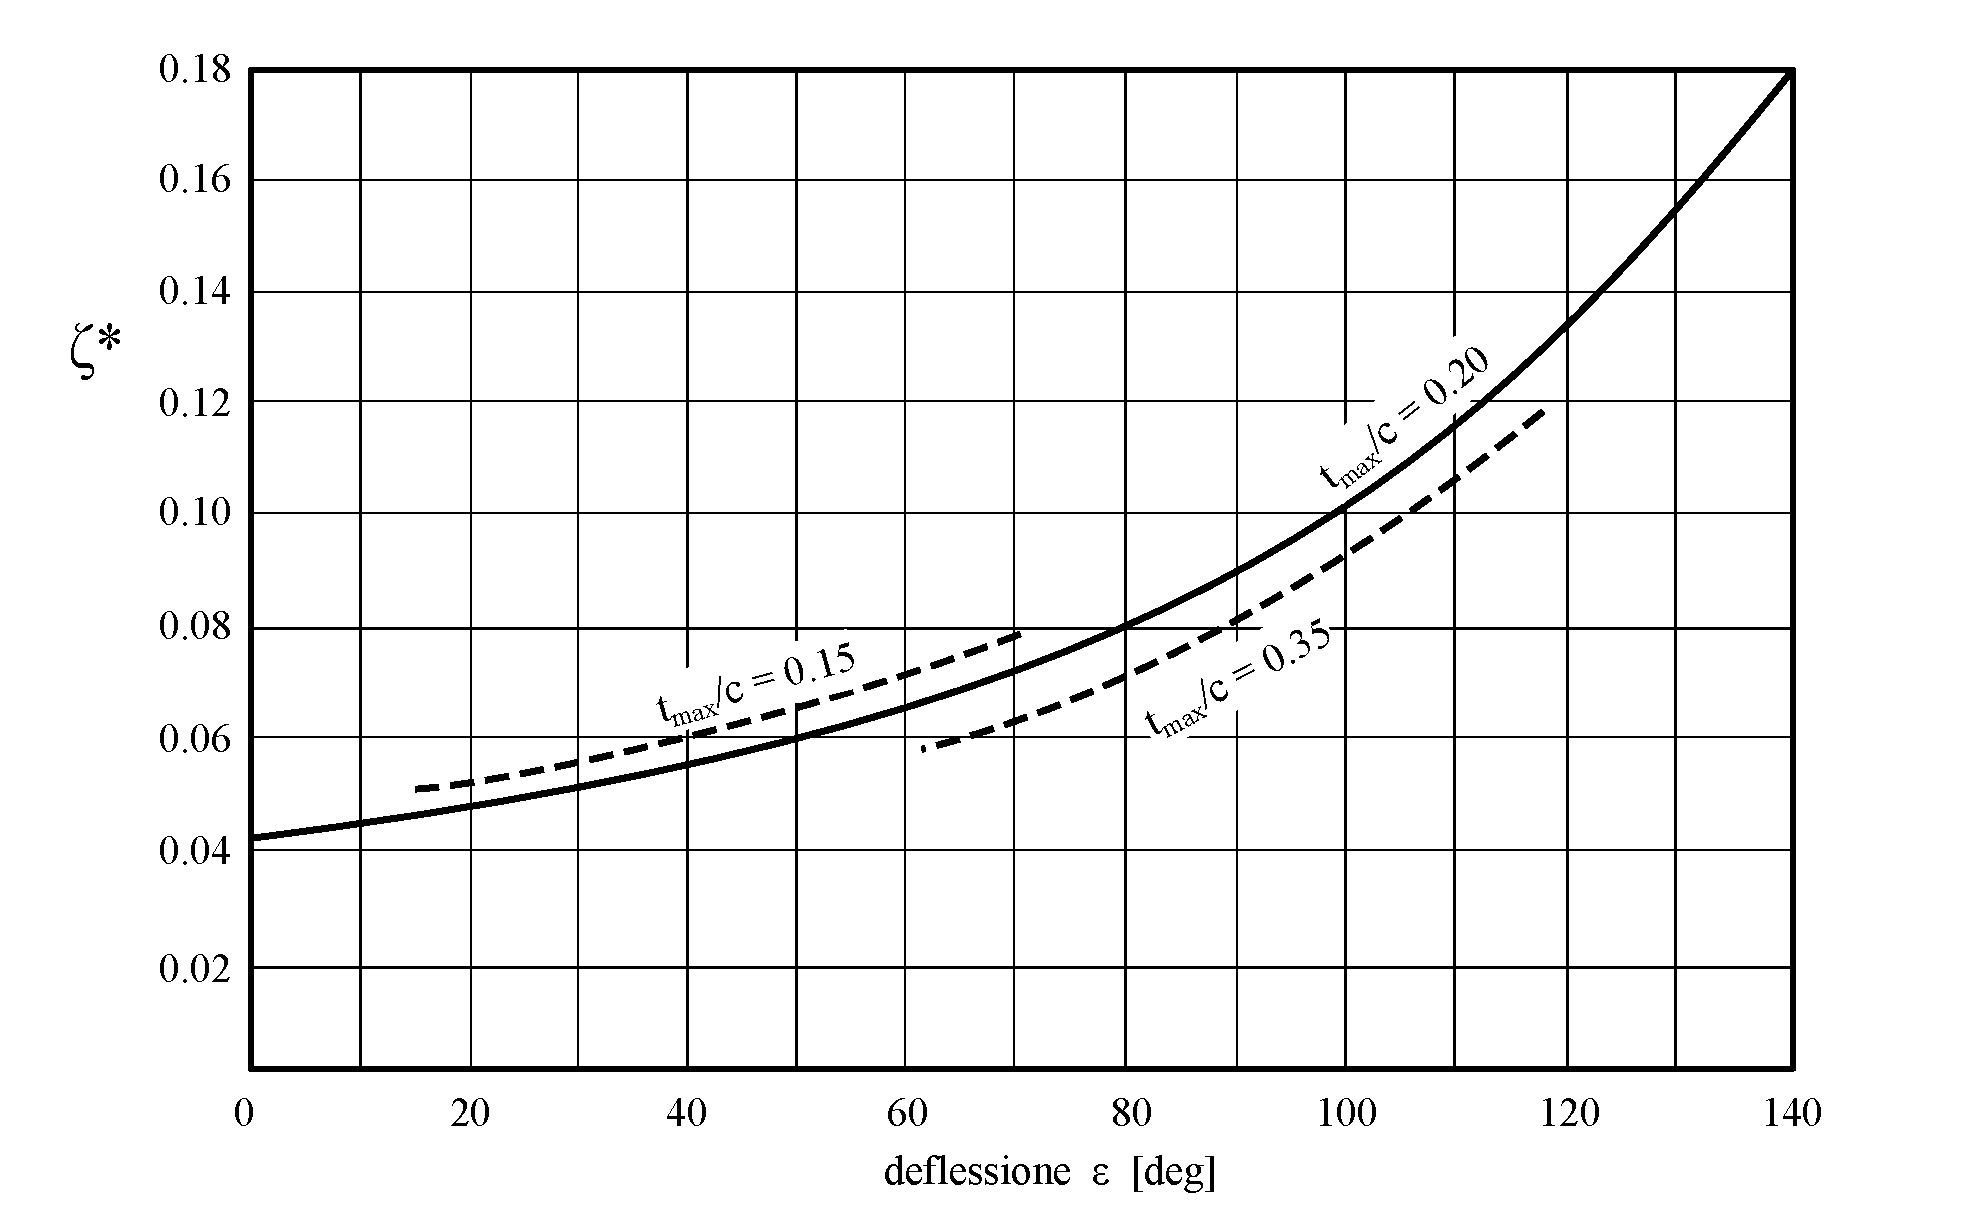
\includegraphics[width=\textwidth]{fig/Soderberg.pdf}
\caption{}
\label{fig:Soderberg}
\end{figure}
\subsection{Ainley-Mathieson}
Si possono vedere anche altre correlazioni come quella di Ainley-Mathieson per la valutazione delle perdite di profilo. Si definiscono dei parametri fissi:
\begin{itemize}
\item $Re = 2 \cdot 10^5$ (basato sulla corda)
\item $M_1 < 0.6$
\item $t_{max}/c = 0.2$
\item $t/s = 0.02$
\item Condizioni nominali (angolo di incidenza nullo)
\end{itemize}
Si definisce il coefficiente di perdita di pressione totale come:
\begin{align*}
Y_P = \frac{p_{0_0} - p_{1_0}}{p_{1_0} - p_1}
\end{align*}
Sperimentalmente la perdita di profilo è definita come:
\begin{align*}
Y_P = \big[ Y_P^* + m_a^2 \left( Y_P^{**} - Y_P^* \right) \big] \Biggl(\frac{\frac{t_{max}}{c}}{0.2} \Biggr)^{m_a}
\end{align*}
con $Y_P^*$ e $Y_P^{**}$ due coefficienti di perdita valutati in due classiche configurazioni di pale:
\begin{align*}
Y_P^* \;\; \to \;\;
\begin{cases}
\alpha_0 = 0\\
R = 0\\
m_a = 0
\end{cases} \hspace{2.5cm}
Y_P^{**} \;\; \to \;\;
\begin{cases}
\alpha_1 = -\alpha_0\\
R = 0.5\\
m_a = 1
\end{cases}
\end{align*}
\begin{align*}
m_a = - \frac{\alpha_0}{\alpha_1} \hspace{1.5cm} 0.15 \leq \frac{t_{max}}{c} \leq 0.25
\end{align*}
\begin{figure}
\centering
  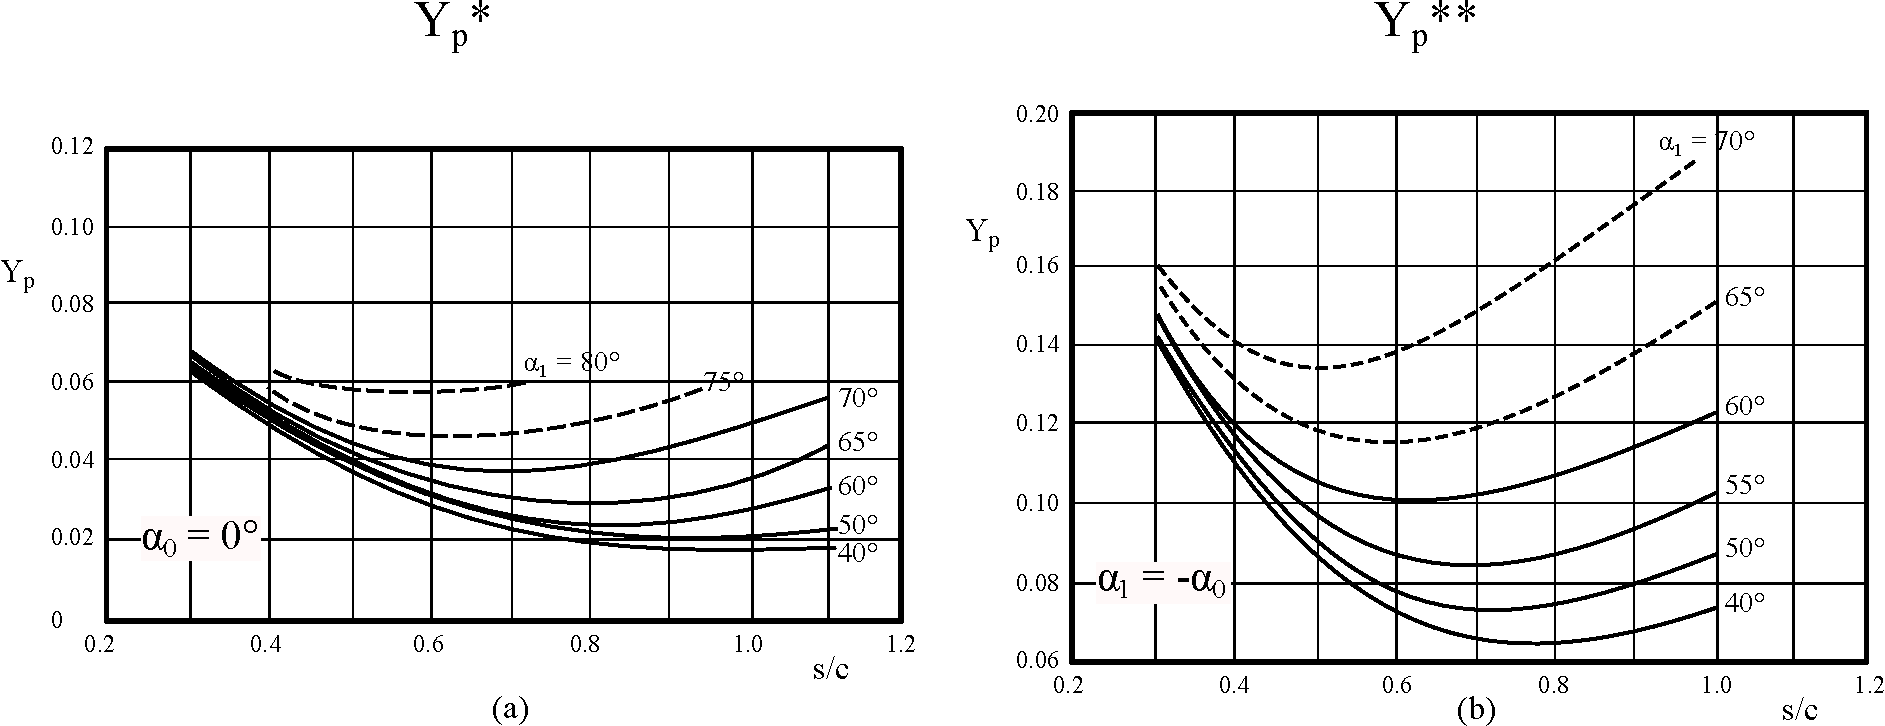
\includegraphics[width=\textwidth]{fig/Mathieson.pdf}
\caption{Perdite di profilo secondo Ainley e Mathieson per ugelli (a) e pale ad azione (b), in condizioni standard.}
\label{fig:Mathieson}
\end{figure}
\\Si possono quindi esprimere le correlazioni corrette:\\
\begin{tabular}{l l}
	$ Y_P = Y_{P,0.02} \bigg[ 1 + 7 \bigg( \frac{t}{s} - 0.02 \bigg) \bigg] $ & correlazione per spessore uscita diverso da quello standard\\
	$ Y_P = Y_{P,2 \cdot 10^5} \bigg( \frac{2 \cdot 10^5}{Re} \bigg)^{0.2} $ &  correlazione per Re diverso da quello standard\\
\end{tabular}

\vspace{0.5cm}
La precedente correlazione fornisce l'espressione solamente per le perdite di profilo; a queste dovranno essere aggiunte le perdite secondarie e per giochi:
\begin{align*}
Y_S + Y_G = \Big( \lambda + B \frac{\delta}{k} \Big) \Bigg( \frac{c_L}{\frac{s}{c}} \frac{\cos^2 \alpha_1}{\cos^3 \alpha_{\infty}} \Bigg)
\end{align*}
con
\begin{itemize}
\item $B = 0.5$ per pale ``libere", $B = 0.25$ per pale ``cerchiate";
\item $h$ altezza della pala;
\item $\delta$ gioco radiale;
\item $\lambda$ un coefficiente sperimentale in funzione di $\Theta$ secondo il grafico \ref{fig:lambdaPerditeSchiera}. $\Theta$ è definito come:
\end{itemize}
\begin{align*}
\Theta = \cfrac{\bigg(\cfrac{A_1}{A_0}\bigg)^2}{1- \cfrac{D_i}{D_e}}
\end{align*}
\begin{figure}
\centering
  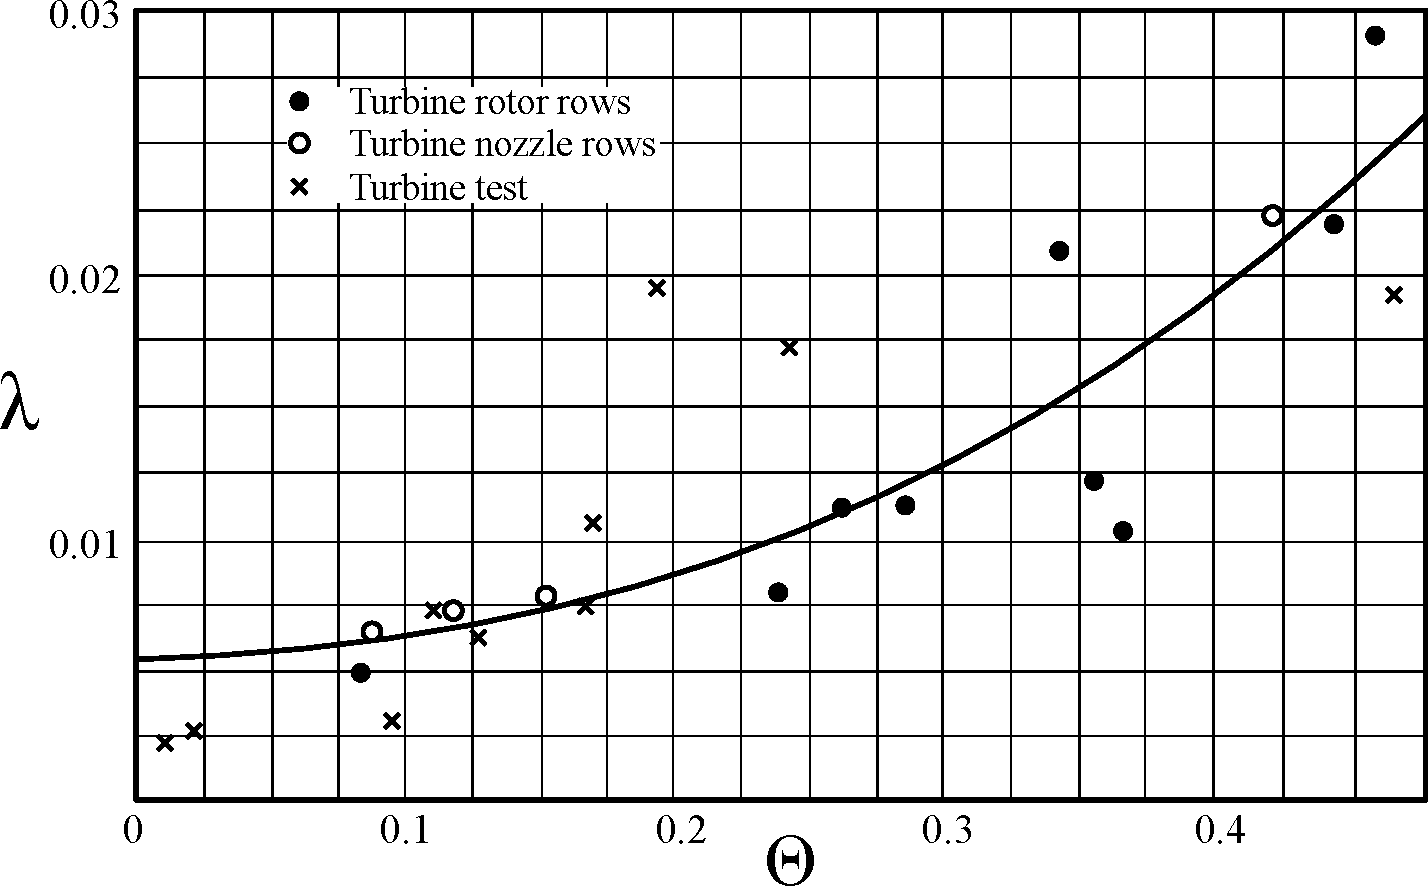
\includegraphics[width=.6\textwidth]{fig/lambdaPerditeSchiera.pdf}
\caption{}
\label{fig:lambdaPerditeSchiera}
\end{figure}

In questo modo si vanno quindi a calcolare le perdite in condizioni fuori progetto usando correlazioni come quelle riportate in figura \ref{fig:FuoriProgT1}.
\begin{figure}
\centering
  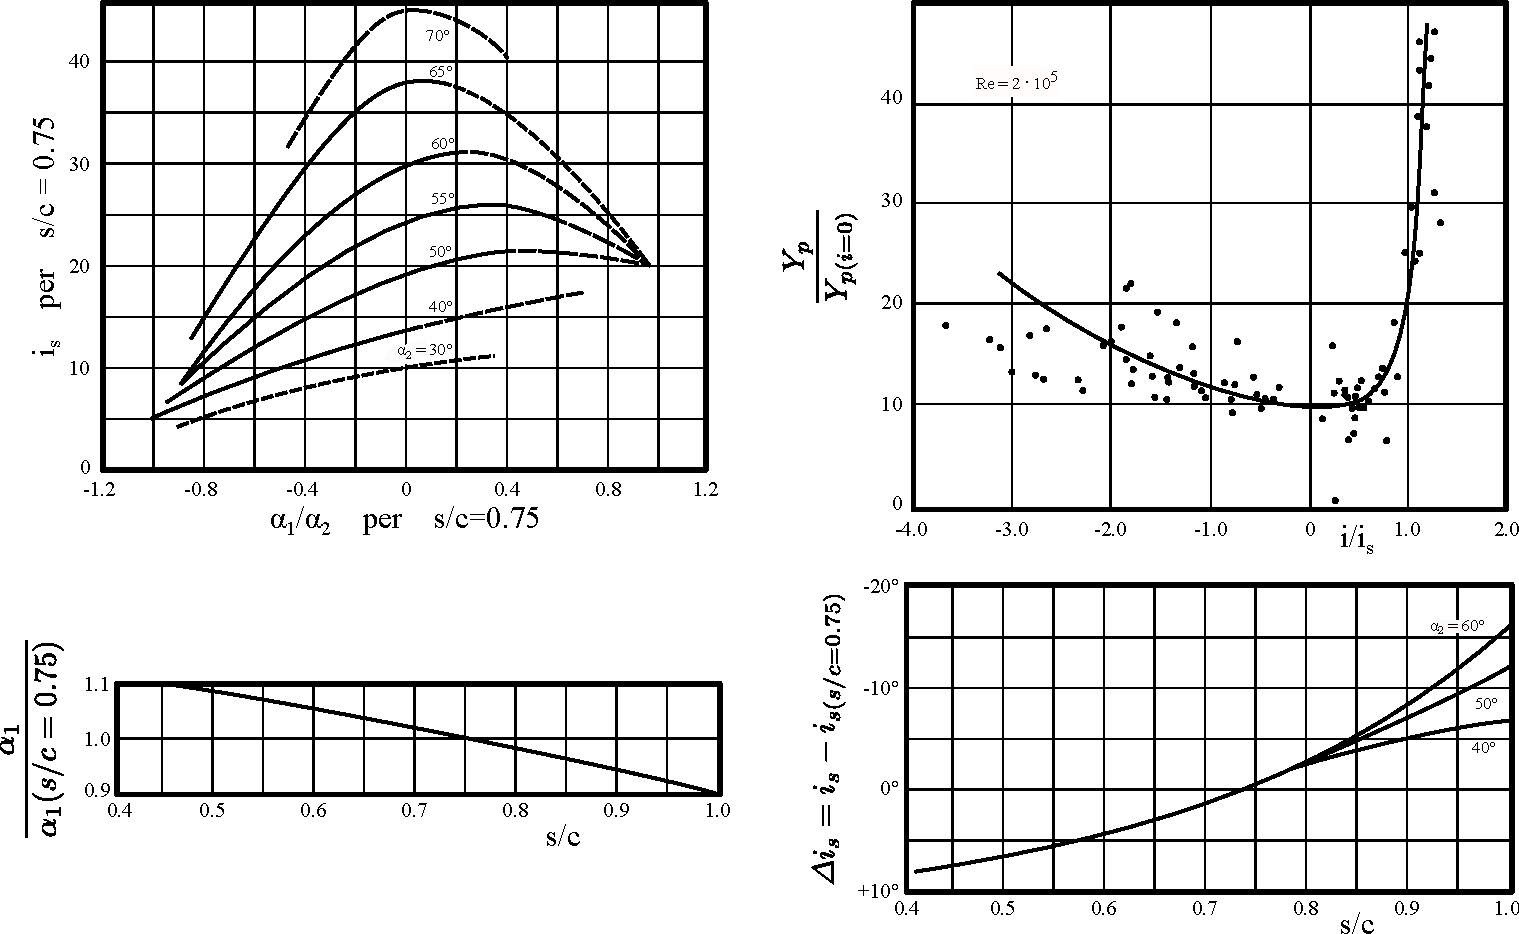
\includegraphics[width=\textwidth]{fig/FuoriProgT1.pdf}
\caption{}
\label{fig:FuoriProgT1}
\end{figure}

\section{Criteri di carico}
\begin{figure}[h!]
\centering
  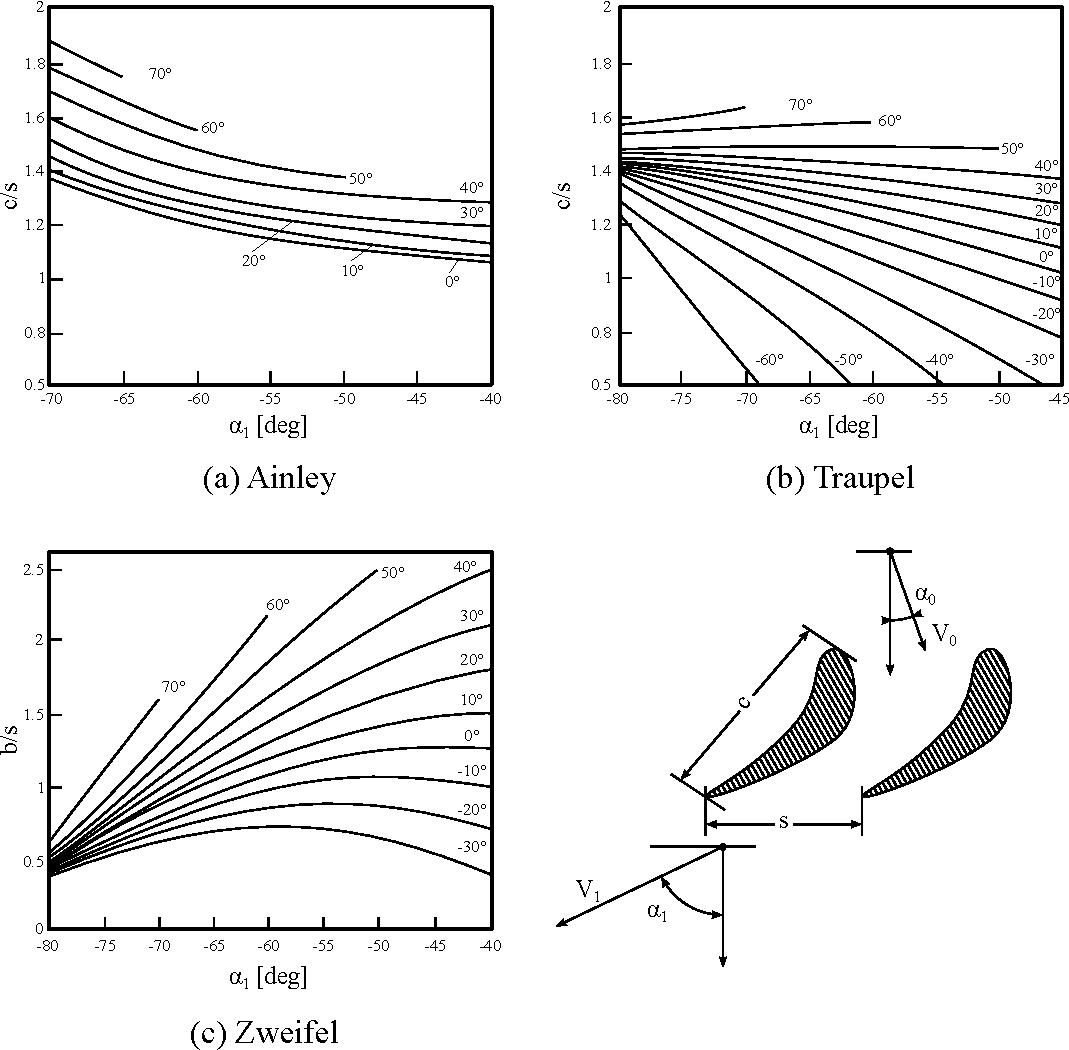
\includegraphics[width=0.95\textwidth]{fig/Ainley.pdf}
\caption{}
\label{fig:Ainley}
\end{figure}
Una volta determinata la schiera è opportuno verificare con un criterio di carico se la solidità scelta è sostenibile o meno. Per esempio con molte pale aumentano le perdite perché aumenta la superficie bagnata ma per contro si riesce a realizzare meglio la variazione d'angolo che è quella che da momento alla turbina.

In figura \ref{fig:Ainley} sono illustrati i diversi criteri di carico. I criteri di Zweifel impongono un vincolo sul rapporto tra forza tangenziale e una forza tangenziale ideale:
\begin{align*}
\cfrac{F_t}{F_{t,id}} = \cfrac{F_t}{\cfrac{1}{2} \rho b c_1^2} = c_{F_t} = 2 \cos^2 \alpha_1 \bigg(\cfrac{c_{m0}}{c_{m1}} \tan \alpha_0 - \tan \alpha_1 \bigg) \cfrac{s}{b} = 0.8
\end{align*}
In figura \ref{fig:CritCaricoT} è rappresentata in rosso l'area formata dall'andamento delle pressioni ideali nell'attraversamento del fluido nel canale interpalare; viene poi evidenziata l'area formata dall'andamento reale in grigio scuro. Il loro rapporto è appunto il rapporto tra le forze tangenziali.
\begin{figure}[h!]
\centering
  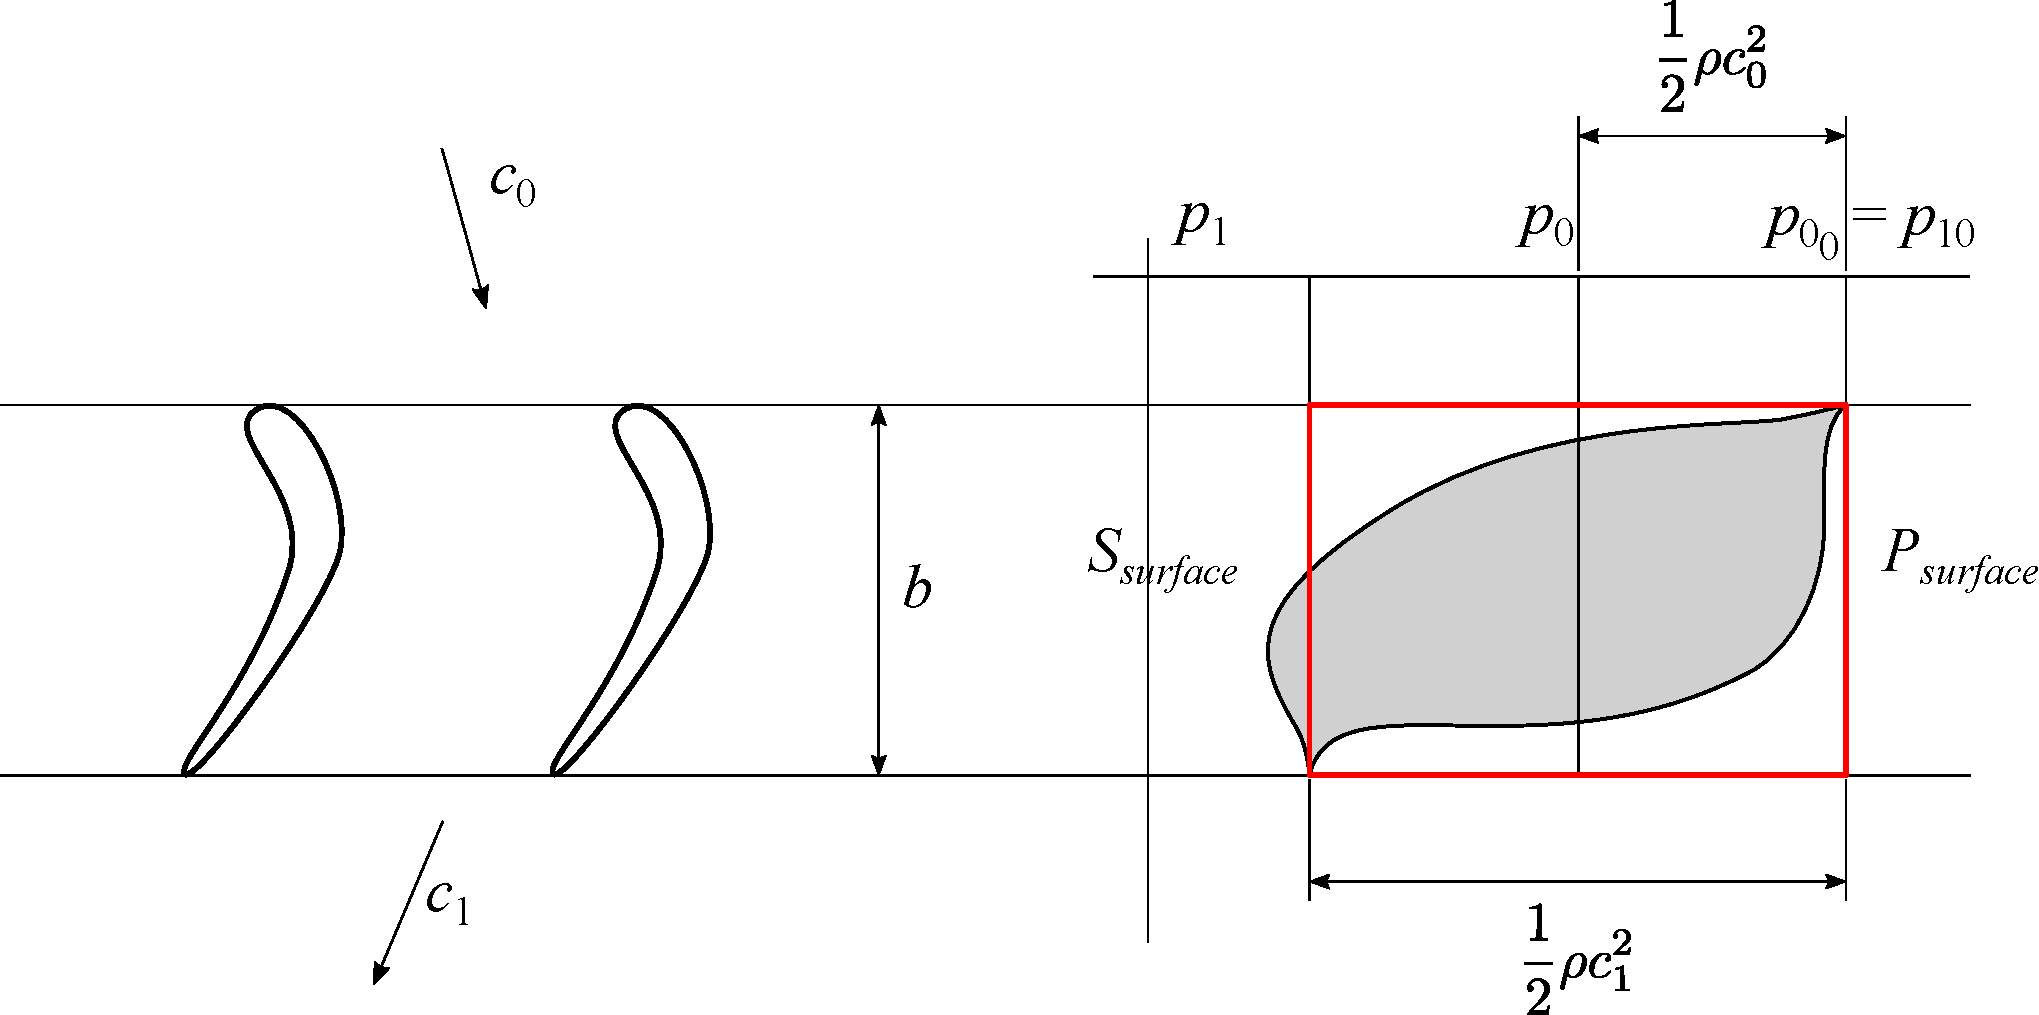
\includegraphics[width=0.95\textwidth]{fig/CritCaricoT.pdf}
\caption{}
\label{fig:CritCaricoT}
\end{figure}